% -*- mode:flyspell; mode:latex -*-
% \documentclass[a4paper,twoside,11pt]{book}
\documentclass[12pt]{article}
\usepackage[latin1]{inputenc}
\usepackage[T1]{fontenc}
\usepackage[english]{babel}
\usepackage{graphicx}
\usepackage{float}
\usepackage{amsmath}
\usepackage{hyperref}
\usepackage{hhline}
\usepackage{subfig}
\usepackage{color}
\usepackage[all]{hypcap}
% \usepackage[normalem]{ulem}  % for striking out
% \usepackage{fancyhdr}
% \pagestyle{fancy}
% \fancyhead[C]{}
% \fancyhead[L] {\it{Mu2e-doc-4555-v1.0} }

\usepackage[square,sort,comma,numbers]{natbib}

% \usepackage[backend=biber, style=numeric-comp, sorting=ynt] {biblatex}

% \addbibresource{mu2e_internal_notes.bib}
% \addbibresource{radiative_muon_capture.bib}
% \addbibresource{radiative_pion_capture.bib}

\newcommand {\red}          {\color{red}}
\newcommand {\blue}         {\color{blue}}

\newcommand {\kmax}         {\mbox{$k_{\rm max}$}}
\newcommand {\mubunch}      {$\mu$Bunch}
\newcommand {\MuMinusEPlus} {\mbox{$\mu^- \rightarrow e^+$}}
\newcommand {\ra}           {\mbox{$\rightarrow$}}

\graphicspath{{figures/}}

\begin{document}

\begin{titlepage}
  \begin{flushright}
    \bf {MU2E/PHYSICS/22262} \\
    version 0.0
    \today
  \end{flushright}

  \vspace{1cm}
  
  \begin{center}
    {\Large \bf Understanding the \kmax\ fits of the RMC spectra} 
    
    \vspace{1cm}
    
    E.Diociaiuti (Roma), M.Mackenzie (Northwestern), P.Murat(FNAL)
    
    % \footnote{\texttt{Fermilab; e-mail: murat@fnal.gov}}
    \vspace{0.3cm}
    
    \vspace{0.8cm}                           
  \end{center}

  \begin{abstract}

    This note summarizes our effort to understand published results on kMax fits
    of the RMC spectra. 
%
    We conclude that internal inconsistencies found in the literature make
    it difficult to rely on the results of other experiments when predicting RMC
    background to the search of \MuMinusEPlus\ conversion process.
    
    To reliably predict RMC background to  \MuMinusEPlus, Mu2e needs to have its own
    measurement of the endpoint of the RMC photon spectrum on Al.
    
  \end{abstract}

\end{titlepage}
% \frontmatter
% \chapter*{Abstract}
%
% \addcontentsline{toc}{chapter}{Abstract}
%
% \mainmatter
%
{\tableofcontents}

%%%%%%%%%%%%%%%%%%%%%%%%%%%%%%%%%%%%%%%%%%%%%%%%%%%%%%%%%%%%%%%%%%%%%%%%%%%%%%%
%\chapter{Calibration}
%%%%%%%%%%%%%%%%%%%%%%%%%%%%%%%%%%%%%%%%%%%%%%%%%%%%%%%%%%%%%%%%%%%%%%%%%%%%%%%
\section{ RMC as a background to \MuMinusEPlus\ conversion search }
% 
% \begin{figure}[H]
%   \includegraphics[width=1.05\textwidth]{figures/png/beam_flash_electron_momentum} 
% 
%   \caption{
%    momentum spectrum of the beam flash electrons
%   }
% \end{figure}

Radiative muon capture (RMC) is one of the most important backgrounds to the search for
\MuMinusEPlus\ conversion on nuclei. In case of the Mu2e target of choice, aluminum,
RMC is also the most uncertain one: the expected signal $e^+$ energy, E = 92.32 MeV,
is close enough to the endpoint of the RMC spectrum on aluminum,
$90 \pm 2$ MeV \cite{RMC_1999_PhysRevC.59.2853}, so variations of the endpoint
energy within the experimental errors could result in significant changes
in the RMC background expectations.
%
%% We note that the uncertainty in the RMC background expectations is mostly due to the
%% published experimental uncertainty of 2 MeV - 
The Mu2e energy resolution of about 300-400 keV
is small compared to a $\sim$ 3 MeV difference between the expected signal energy
and the maximal energy of a positron coming from a conversion of a RMC photon.
However, given the published 2 MeV uncertainty on the RMC spectrum endpoint the two 
numbers are just about 1.5 standard deviation apart, so understanding of the
experimental uncertainty on \kmax\ becomes quite important.

Fortunately, measurements of the photon spectra on nuclei published 
by the TRIUMF RMC spectrometer group in \cite{RMC_1992_PhysRevC.46.1094},
\cite{RMC_1999_PhysRevC.59.2853} provide sufficient information for readers
to reproduce the published photon spectrum endpoints, and in this note
we report on our attempt to do so.

The endpoint of the RMC photon spectrum is determined using the closure
approximation model \cite{RMC_1979_CERN_REF-TH-2967}.
In this model, the photon spectrum is fully defined by a single parameter,
the photon spectrum endpoint energy \kmax:
$$
   {dN \over dx} = {e^2 \over \pi} {\kmax^2 \over {m_\mu^2}}  (1-x) (1-2x+2x^2) x (1-x)^2
$$
where $x = k/\kmax$.

We use published parameterizations of the TRIUMF RMC spectrometer response
to convolute them with the closure approximation spectra, fit the experimental data,
determine the best \kmax\ values and the corresponding fit uncertainties
for different nuclei, and compare the fit results to the published values.

%%%%%%%%%%%%%%%%%%%%%%%%%%%%%%%%%%%%%%%%%%%%%%%%%%%%%%%%%%%%%%%%%%%%%%%%%%%%%%%
\section { Parameterization of the Detector Response}

As published RMC spectra have the detector response convoluted in, to compare
them to the model predictions one needs to know the detector response.

Fortunately, the TRIUMF group which has published the most recent highest statistics
RMC spectra, has also made published its detector response -
see \cite{RMC_1992_PhysRevC.46.1094} and \cite{RMC_1998_PhysRevC.58.1767}. 

The detector response D(E,E') is defined as the probability for a photon
with energy E to be reconstructed in the detector with energy E'. As follows from the
definition, D(E,E') includes both resolution and acceptance - the integral of D(E,E')dE'
gives the total acceptance for a given energy E.

In both \cite{RMC_1992_PhysRevC.46.1094} and \cite{RMC_1998_PhysRevC.58.1767}, the
detector response is determined using the GEANT3-based simulation using monoenergetic
photons in a energy range of 50-140 MeV, and parameterized analytically.
The parameterizations of  \cite{RMC_1992_PhysRevC.46.1094} and \cite{RMC_1998_PhysRevC.58.1767}
are significantly different, the source of the difference is not understood.

%%%%%%%%%%%%%%%%%%%%%%%%%%%%%%%%%%%%%%%%%%%%%%%%%%%%%%%%%%%%%%%%%%%%%%%%%%%%%%
\subsection { 1992 Detector response parametrization }

The response of the TRIUMF RMC spectrometer published in \cite{RMC_1992_PhysRevC.46.1094}
is described as a Gaussian function with the exponential low- and  high-energy tails.
In order to reproduce the low-energy resolution tail for high-energy photons, a second Gaussian
is added for the photon energy E>60 MeV. The functional form is as follows:

\begin{equation}
  \label{eq:001}
\text{D(E,E')}= \left\{
\begin{array}{ll}
                \text{A exp}\left[-\frac{1}{2\sigma_0^2}(E'-E_o)^2\right]+
                \text{F exp}\left[-\frac{1}{2\sigma_3^2}(E'-E_3)^2\right]
 \quad E_1<E'<E_2 \\
                \text{B exp}\left[-\frac{1}{\sigma_1}(E_1-E') \right]+
                \text{F exp}\left[-\frac{1}{2\sigma_3^2}(E'-E_3)^2\right]
 \quad E'<E_1      \\  
                \text{C exp}\left[-\frac{1}{\sigma_2}(E'-E_2)\right]+
                \text{F exp}\left[-\frac{1}{2\sigma_3^2}(E'-E_3)^2\right]
 \quad E'>E2     
 \end{array}
 \right\}
\end{equation}
 
where $E_1=E_0 - \frac{\sigma_0^2}{\sigma_1}$, $E_2 =E_0 + \frac{\sigma_0^2}{\sigma_2}$,
 $B=\text{A exp}\left[-\frac{\sigma_0^2}{2\sigma_1^2}\right]$, 
 $C=\text{A exp}\left[\frac{\sigma_0^2}{2\sigma_2^2}\right]$. 

 The parameters $A, B ,C , F, \sigma_i$  etc are fitted as polynomials in the photon energy:
 
\begin{equation}
  f(E)= P_0+P_1E+P_2E^2+P_3E^3
\end{equation}

The coefficients are reported in tables ~\ref{tab:coefficients1} and ~\ref{tab:coefficients2} .

\begin{table}[!h]
\begin{center}
\begin{tabular}{| c | c | c | c | c | }
\hline
Parameter & $P_0$ (MeV)& $P_1$ & $P_2$ (MeV)$^{-1}$ \\ \hline
$\sigma_0$ & -0.5836 & 0.0352 & \\ \hline
$\sigma_1$ & -5.879 & 0.1653 & -5.149$\times 10^{-4}$ \\ \hline
$\sigma_2$ & 1.596 & -0.03859 & 3.883$\times 10^{-4}$ \\ \hline
$\sigma_3$ & -47.80 & 1.010 & -4.406$\times 10^{-3}$ \\ \hline
E$_3$ & 1.068 & 0.7507 & \\ \hline
E$_0$ (E>60) & -1.161 & 0.9481 & 1.724$\times 10^{-3}$ \\ \hline
E$_0$ (E<60) & 22.73 & 0.1995 & 5.993$\times 10^{-3}$ \\ \hline

\end{tabular}
\end{center}
\caption{
  Polynomial parameterization of the coefficiencts in \ref{eq:001}
  \label{tab:coefficients1}}
\end{table}

\begin{table}[!h]
\begin{center}
\begin{tabular}{| c | c | c | c | c | c |}
\hline
Parameter & $P_0$ & $P_1$ (MeV)$^{-1}$ & $P_2$ (MeV)$^{-2}$  & $P_3$ (MeV)$^{-3}$\\ \hline
A & 3.259$\times 10^{-4}$ & -4.120$\times 10^{-4}$ & 1.015$\times 10^{-5}$ & -4.05$\times 10^{-8}$  \\ \hline
F/A & -0.1337 & 2.828$\times 10^{-3}$ & -9.701$\times 10^{-6}$ & \\ \hline
\end{tabular}
\end{center}
\caption{Polynomial parameterization of coefficients in \label{tab:coefficients2}}
\end{table}

The energy dependence of several coefficients used to parameterize the response
function is shown in Fig.~\ref{fig:parameterDependence}.

\begin{figure}[!h]
  \begin{center}
    \includegraphics[width=0.33\columnwidth]{png/sigmas92.png} 
    \includegraphics[width=0.33\columnwidth]{png/A_FoverA92.png} 
    \includegraphics[width=0.33\columnwidth]{png/E092.png} 
  \end{center}
  \caption{
    Energy dependence of parameters defining the TRIUMF RMC spectrometer response
    \cite{RMC_1992_PhysRevC.46.1094}
  }
  \label{fig:parameterDependence}
\end{figure}

Examples of the detector response at different energies, namely, \mbox{50 MeV},
70 MeV , 90 MeV, and 110 MeV, are shown in Fig.~\ref{fig:92ResponseExample}.

As previously described, for photon energies E>60 MeV, the low-energy tails are well evident.

\begin{figure}[!h]
\centering
\includegraphics[width =\textwidth]{png/Resp_example92.png}
\caption{'1992 detector response parametrization for different photon energies}
\label{fig:92ResponseExample}
\end{figure}


\subsection { 1998 Detector Response }

The TRIUMF RMC spectrometer response published in 1998 (\cite{RMC_1998_PhysRevC.58.1767})
is significantly different from its '1992 version.
The '1998 parameterization is a gaussian with logaritmic low-energy and an exponential
high-energy tails:

\begin{equation}
  D(E,E')= \left\{
    \begin{array}{ll}
      \beta \cdot ln(x)/x    \qquad E' \leq (E_0-\sigma_0) \\
      Ae^{-(E'-E_0)^2/2\sigma_0^2} \qquad E0-\sigma_0<E'<(E_0-\sigma_0^2/\sigma^2) \\
      Ae^{-(E'-E_0)/2\sigma_2}    \qquad E' \geq (E_0+\sigma_0^2/\sigma_2)
    \end{array}
  \right\}
\end{equation}

The parameter $\beta$  allows to match the low-side and the gaussian core
of the distribution at E'=$E_0-\sigma_0$.
$x$ is defined as
$$
  x= \frac{\alpha- E'}{\alpha -37} 
$$, E in MeV.
Dependence of the coefficients $\alpha, A, E_0, \sigma_0, \sigma_2$ on the photon energy
is parameterized with the 3-rd order polinomials:

\begin{equation}
  \alpha= a_0+a_1y+a_2y^2+a_3y^3
\end{equation}

where $y= (E-60)/60$, E in MeV.

Polinomial coefficients which parameterize the energy dependence of
$\alpha, A, E_0, \sigma_0, \sigma_2$ are presented in Tab.~\ref{tab:param98}

\begin{table}[!h] \label{tab:param98}
  \begin{center}
    \begin{tabular}{| c | c | c | c | c | c | }
      \hline
      Parameter  & $a_0$              & $a_1$ & $a_2$ & $a_3$ \\ \hline
      $\alpha$   & 56.1               &62.5 & -0.826 & 0.0  \\ \hline
      A          & 9.41$\cdot 10^{-4}$ & 2.61$\times 10^{-3}$ &0.27 $\times 10^{-2}$ &0.835$\times 10^{-3}$   \\ \hline
      $E_0$      & 54.4               & 57.7 & -0.315 &0.0 \\ \hline
      $\sigma_0$ & 2.03               &10.4 &1.25 & -0.428\\ \hline
      $\sigma_2$ & 0.786              & 0.508 & 0.425 & -0.164\\ \hline
    \end{tabular}
  \end{center}
  \caption{Coefficients used to parameterize the energy dependence of the response function parameters}
\end{table}

Figure~\ref{fig:parameters98} shows the energy dependence of the coefficients used
in the detector response function parameterization.

\begin{figure}[!h]
  \begin{center}
    \includegraphics[width=0.49\columnwidth]{png/sigmas98.png} 
    \includegraphics[width=0.49\columnwidth]{png/par98.png} 
  \end{center}
  \caption{Energy dependence of the different parameter defining the detector response}
  \label{fig:parameters98}
\end{figure}

Figure~\ref{fig:response98} shows the '1998 detector response for four different photon energies.

The distributions in Figure~\ref{fig:response98} are significantly wider than similar distributions
shown in Figure~\ref{fig:92ResponseExample}. Given that there were no big reported changes in the TRIUMF
RMC spectrometer configuration, one can conclude that understanding of the detector response has
significantly evolved in between 1992 and 1998. However, there is no corresponding discussion 
in the '1998 paper. 

\begin{figure}[!h]
\centering
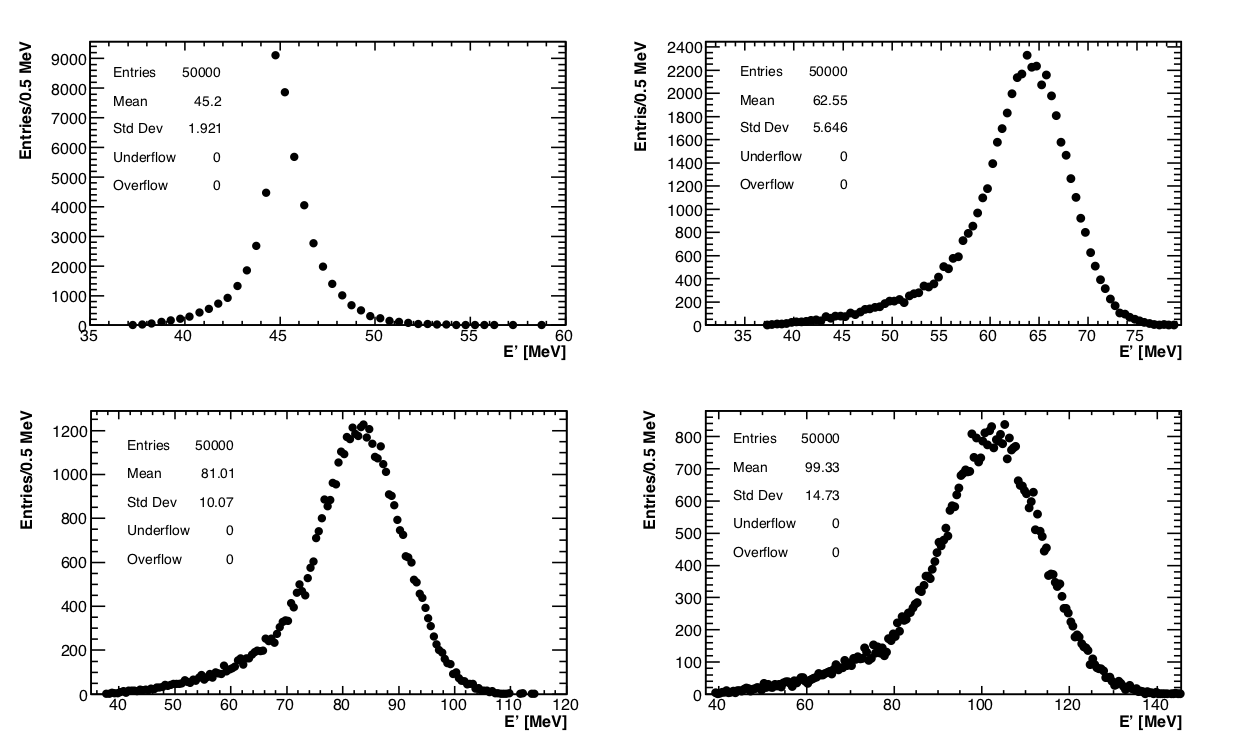
\includegraphics[width =\textwidth]{png/Resp_example98.png}
\caption{1998 detector response parametrization for different photon energies}
\label{fig:response98}
\end{figure}

Figure~\ref{fig:shapecomp} compares the '1992 and '1998 versions of the
TRIUMF RMC spectrometer response at $E_{\gamma}=90$ MeV (left) and 
the linearity of the detector response for '1992 and '1998 version
as a function of the photon energy (right).

\begin{figure} [!h]
\centering
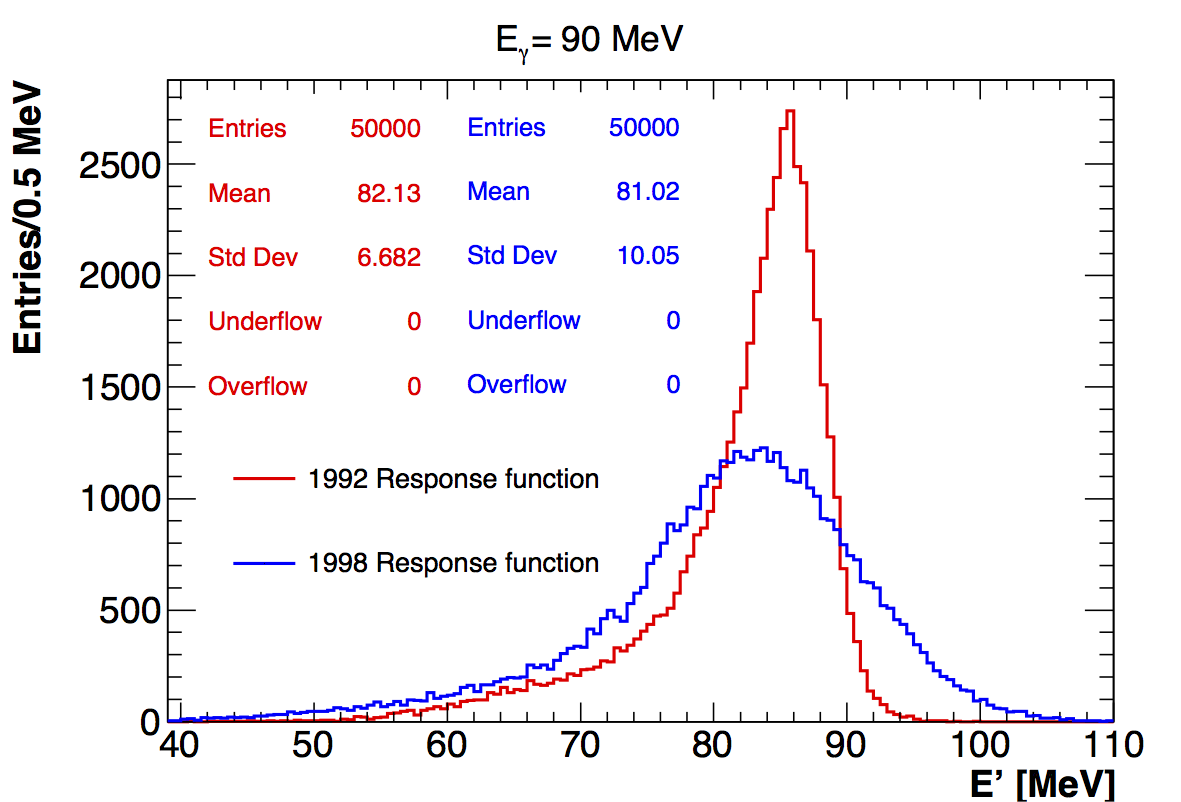
\includegraphics[width=0.49\columnwidth]{png/detRespinsieme.png}
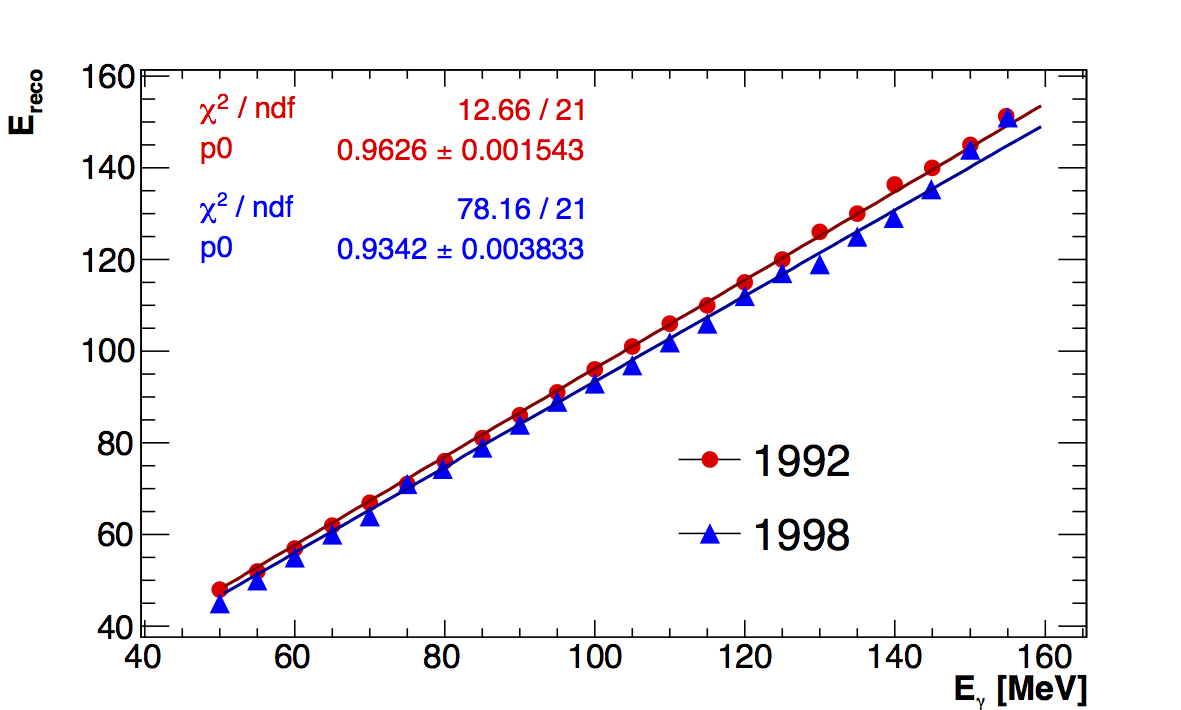
\includegraphics[width=0.49\columnwidth]{png/9298fit.png}
\caption{
  Left: '1992 and '1998 detector response at $E_{\gamma}=90$ MeV.
  Right: dependence of the peak of the detector response function on $E_{\gamma}$
  for '1992 and '1998 response parameterizations.
}
\label{fig:shapecomp} 
\end{figure}

Figure ~\ref{p004} shows how well the '1992 and '1998 parameterizations of the detector
response describe the radiative pion capture (PRC) peak on hydrogen at E = 129.4 MeV
from $\pi^{-}p \rightarrow \gamma n$ on LH$_{2}$ reactiion reported in the '1992 paper.
Figure ~\ref{p004} demonstrates that the modeled '1992 detector response is consistent
with the '1992 data, and the difference between the two parameterizations can't be
interpreted in terms of improved , from 1992 to 1998, understanding of the detector
response.\\

  \begin{figure}[!h]
 \begin{center}
 \includegraphics[width=0.49\columnwidth]{png/RPC_Data_vs_1992_Response.png} 
 \includegraphics[width=0.49\columnwidth]{png/RPC_Data_vs_1998_Response.png} 
 \end{center}
 \caption{Response function of the 1992 article (left) and 1998 article (right) compared with the 129.4 MeV line from RPC on LH$_{2}$}
 \label{p004}
 \end{figure}

 The '1998 article also validates the detector response, showing the MC description of the
 photon spectrum from RPC on $^{12}$Ca  - see Figure~\ref{fig:art9}. However, this distribution
 is wide so the '1998 data-to-MC comparison is less sensitive to the modeled detector resolution
 than the '1992 comparison.

\begin{figure}[!h]
 \begin{center}
 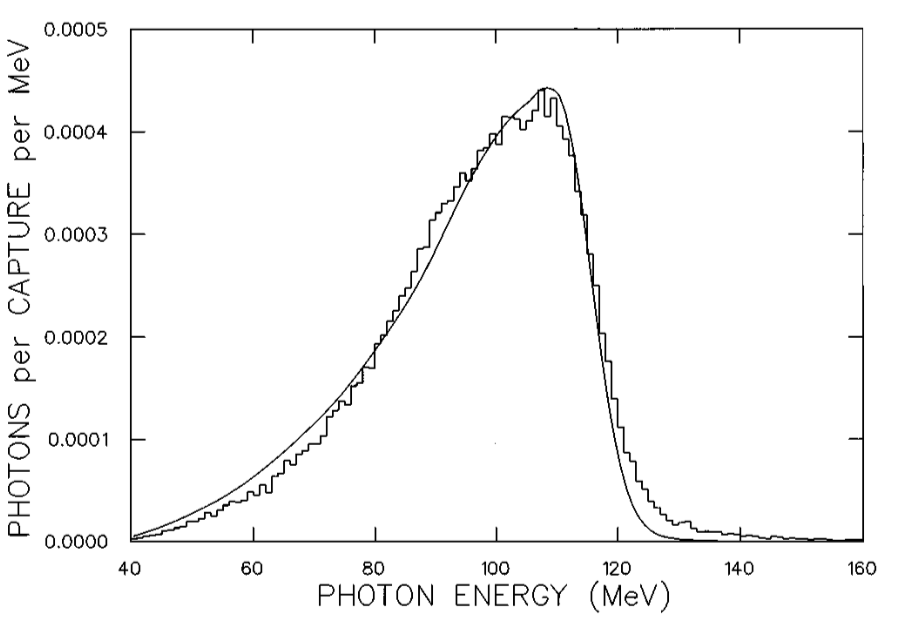
\includegraphics[width=0.45\textwidth]{png/RPC12Ca.png} 
 \end{center}
 \caption{RPC spectrum from  $\pi^{-}p \rightarrow \gamma n$ on  $^{12}$Ca compared to the simulated data }
 \label{fig:art9}
 \end{figure}

%%%%%%%%%%%%%%%%%%%%%%%%%%%%%%%%%%%%%%%%%%%%%%%%%%%%%%%%%%%%%%%%%%%%%%%%%%%%%%%
\section { Input data for the \kmax\ fits}

The digitized figures from references \cite{RMC_1992_PhysRevC.46.1094,RMC_1999_PhysRevC.59.2853}
are used as input data for our fits. We assume that the published spectra plot numbers of events
per bin and that the errors used in the fits are purely statistical.

To check the first assumption, we show in Figure \ref{fig:digitization_accuracy_x_y_left} the accuracy
of digitizing the energy bin centers for a digitized plot. It is calculated as the difference between 
the digitized bin center and the expected bin center, N+0.5.
Figure \ref{fig:digitization_accuracy_x_y_right} shows the accuracy of digitizing the bin contents.
Plotted is the difference between the digitization and the closest integer, where the assumption is that 
each bin contains an integer number of entries. The digitization accuracy of the bin contents has
a standard deviation close to 0.1 and a mean also close to 0.1, which could be due to a
mis-calibration of the Y axis in the digitization of the plot.

\begin{figure}[htbp]
  \begin{center}
    \subfloat[\label{fig:digitization_accuracy_x_y_left}]{ %
    \includegraphics[width=0.49\columnwidth]{png/digitization_accuracy_de}}
    \subfloat[\label{fig:digitization_accuracy_x_y_right}]{ %
    \includegraphics[width=0.49\columnwidth]{png/digitization_accuracy_Al_1992_dy} }
  \end{center}
  \caption{
    (a): accuracy of digitizing the histogram bin centers
    (b): digitization accuracy of the bin content
  }
  \label{fig:digitization_accuracy_x_y}
\end{figure}

The distribution in figure \ref{fig:digitization_accuracy_error_bars} plots the residuals
$\Delta_Y = 0.5((Y+\sigma_Y) + (Y-\sigma_Y)) - \sqrt{Y}$ for one of the digitized plots.
It confirms the assumption that the error bars on the plots are purely statistical.

\begin{figure}[htbp]
  \begin{center}
    \includegraphics[width=0.99\columnwidth]{png/digitization_error_bars} 
  \end{center}
  \caption{
    left: error bar residuals, $\Delta_Y$, vs the digitized error bars
    right: y-projection of the left histogram
  }
  \label{fig:digitization_accuracy_error_bars}
\end{figure}


\section { Systematic uncertainty on the energy scale}

The energy scale of the TRIUMF RMC spectrometer has been calibrated using the
radiative pion capture (RPC) on hydrogen \cite{RMC_1992_WRIGHT_1992_249}.
Figure \ref{fig:1992_photon_spectrum_calibration} shows the measured RPC spectrum
overlayed with the simulation results. The histogram bin width
is 500 keV, and one can see that the systematic uncertainty in the reconstructed
photon energy does not exceed one bin, i.e. 0.5 MeV. Differences near 80 MeV
more likely reflect systematic error in the acceptance calculation.

\begin{figure}[htbp]
  \begin{center}
    \includegraphics[width=0.7\columnwidth]{png/1992_TRIUMF_RMC_facility_fig_9_photon_spectrum_calibration} 
  \end{center}
  \caption{
    RPC spectrum on hydrogen measured at the TRIUMF RMC spectrometer \cite{RMC_1992_WRIGHT_1992_249}.
    In the region of the RPC peak, the systematic uncertainty in the reconstructed photon energy does
    not exceed one bin, i.e. 500 keV.
  }
  \label{fig:1992_photon_spectrum_calibration}
\end{figure}

%%% Local Variables:
%%% mode: latex
%%% TeX-master: "."
%%% End:

%%%%%%%%%%%%%%%%%%%%%%%%%%%%%%%%%%%%%%%%%%%%%%%%%%%%%%%%%%%%%%%%%%%%%%%%%%%%%%% 
%%% Local Variables:
%%% mode: latex; mode: flyspell
%%% TeX-master: "."
%%% End:

\section { Fits }

To fit the end point value, convolved spectrums were generated for end point energies
between 80 MeV and 100 MeV using both detector response functions. The spectrums were scaled to minimize the $\chi^2$
or the negative log likelihood ($\mathcal{L}$), where the latter is able to take into account empty
bins in the data while the former cannot. For the $\mathcal{L}$, the convolved spectrum value was taken as the mean of
a Poisson distribution. The scale factors to minimize the $\chi^2$ and $\mathcal{L}$ fits were derived by:

$$f_{Poisson}(N;x_i) = \frac{x_i^N e^{-x_i}}{N!}$$
$$\chi^2 = \sum^N_{i=1} (\frac{A*x_i - y_i}{\sigma_i})^2; \mathcal{L} = -\sum^N_{i=1}log(f_{Poisson}(y_i;A*x_i))$$
$$\frac{\partial \mathcal{L}}{\partial A} = 0 \rightarrow A_{\mathcal{L}} = \frac{\sum^N_{i=1} y_i}{\sum^N_{i=1} x_i} $$
$$\frac{\partial \chi^2}{\partial A} = 0 \rightarrow A_{\chi^2} = \frac{\sum^N_{i=1} \frac{x_i*y_i}{\sigma_i^2}}{\sum^N_{i=1} \frac{x_i^2}{\sigma_i^2}} $$

\noindent
where $x_i$ is the predicted value corresponding to data $y_i$ for a given end point value.

The distribution of $\chi^2$ and $\mathcal{L}$ values as a function of the end point energy were each fit to a parabola near 
the minimum using ROOT to find the best fit end point value. The estimated uncertainty on the end point energy is then
defined by $\Delta \chi^2 = 1$ and $\Delta \mathcal{L} = \frac{1}{2}$. An example fit using the 1992 detector response function
and the 1992 aluminum data is shown in figure \ref{fig:1992AlFits}. The fit end point values for all 
datasets and both detector response functions are shown in figures \ref{fig:ChiSq} and \ref{fig:NLL}, and the $\chi^2$/DoF
distribution is shown in figure \ref{fig:ChiSqOfFits}. The $\chi^2$/DoF peaks around 1 for the 1998 detector response 
function and does not have the expected shape for the 1992 detector response function. Figure \ref{fig:compareFits}
shows the difference between these fits. Figure \ref{fig:ToyFitErrs} shows the errors in fitting toy data generated with
an end point value of 90 MeV. The toy fits shows that the expected difference between the $\chi^2$ and $\mathcal{L}$ fits is around 0.5 MeV.
The difference between the two fits for the data is around 1 MeV for the fits using the 1998 detector response function,
which is larger than expected but not too far off. The difference between the fits when using the 1992 detector response function
is around 3 MeV, consistent with the 1992 detector response not describing the data well.
The toy data fits suggests that the $\mathcal{L}$ fit end point values are closer to the true value due to a bias of around 0.5 MeV 
in the $\chi^2$ fits.

%%  where the $\mathcal{L}$ fit end point values are consistently higher which is consistent
%% with $\mathcal{L}$ being more sensitive to bins with low entries.

%% The published data was fit using both of the published response functions.
%% The method to fit the data was to minimize the $\chi^2$ value for many values
%% of kMax, and then fit a parabola to the $\chi^2$ distribution, 
%% $\chi^2_{Min} + \frac{(k-kMax)^2}{\sigma^2}$. The uncertainty on the fit kMax
%% is then the inverse square root of the coefficient. This was also done using
%% a negative log likelihood ($\mathcal{L}$) minimization strategy, where the variance is half of
%% the inverse of the leading coefficient. 
%% The latter is able to take into account empty
%% bins in the data while the former cannot. The end point values for each target Z 
%% are shown in figure \ref{fig:ChiSq} and \ref{fig:NLL} using $\chi^2$ and $\mathcal{L}$ minimization
%% respectively, and the $\chi^2$/DoF is shown in figure \ref{fig:ChiSqOfFits}. The $\mathcal{L}$
%% fitting method includes empty bins, which are ignored by the $\chi^2$ fitting method,
%% and has a greater cost for deviating from bins with small entry numbers. This results
%% in the $\mathcal{L}$ fit end point values being consistently higher, as is shown in figure \ref{fig:compareFits}.

\begin{figure}[h]
  \centering
  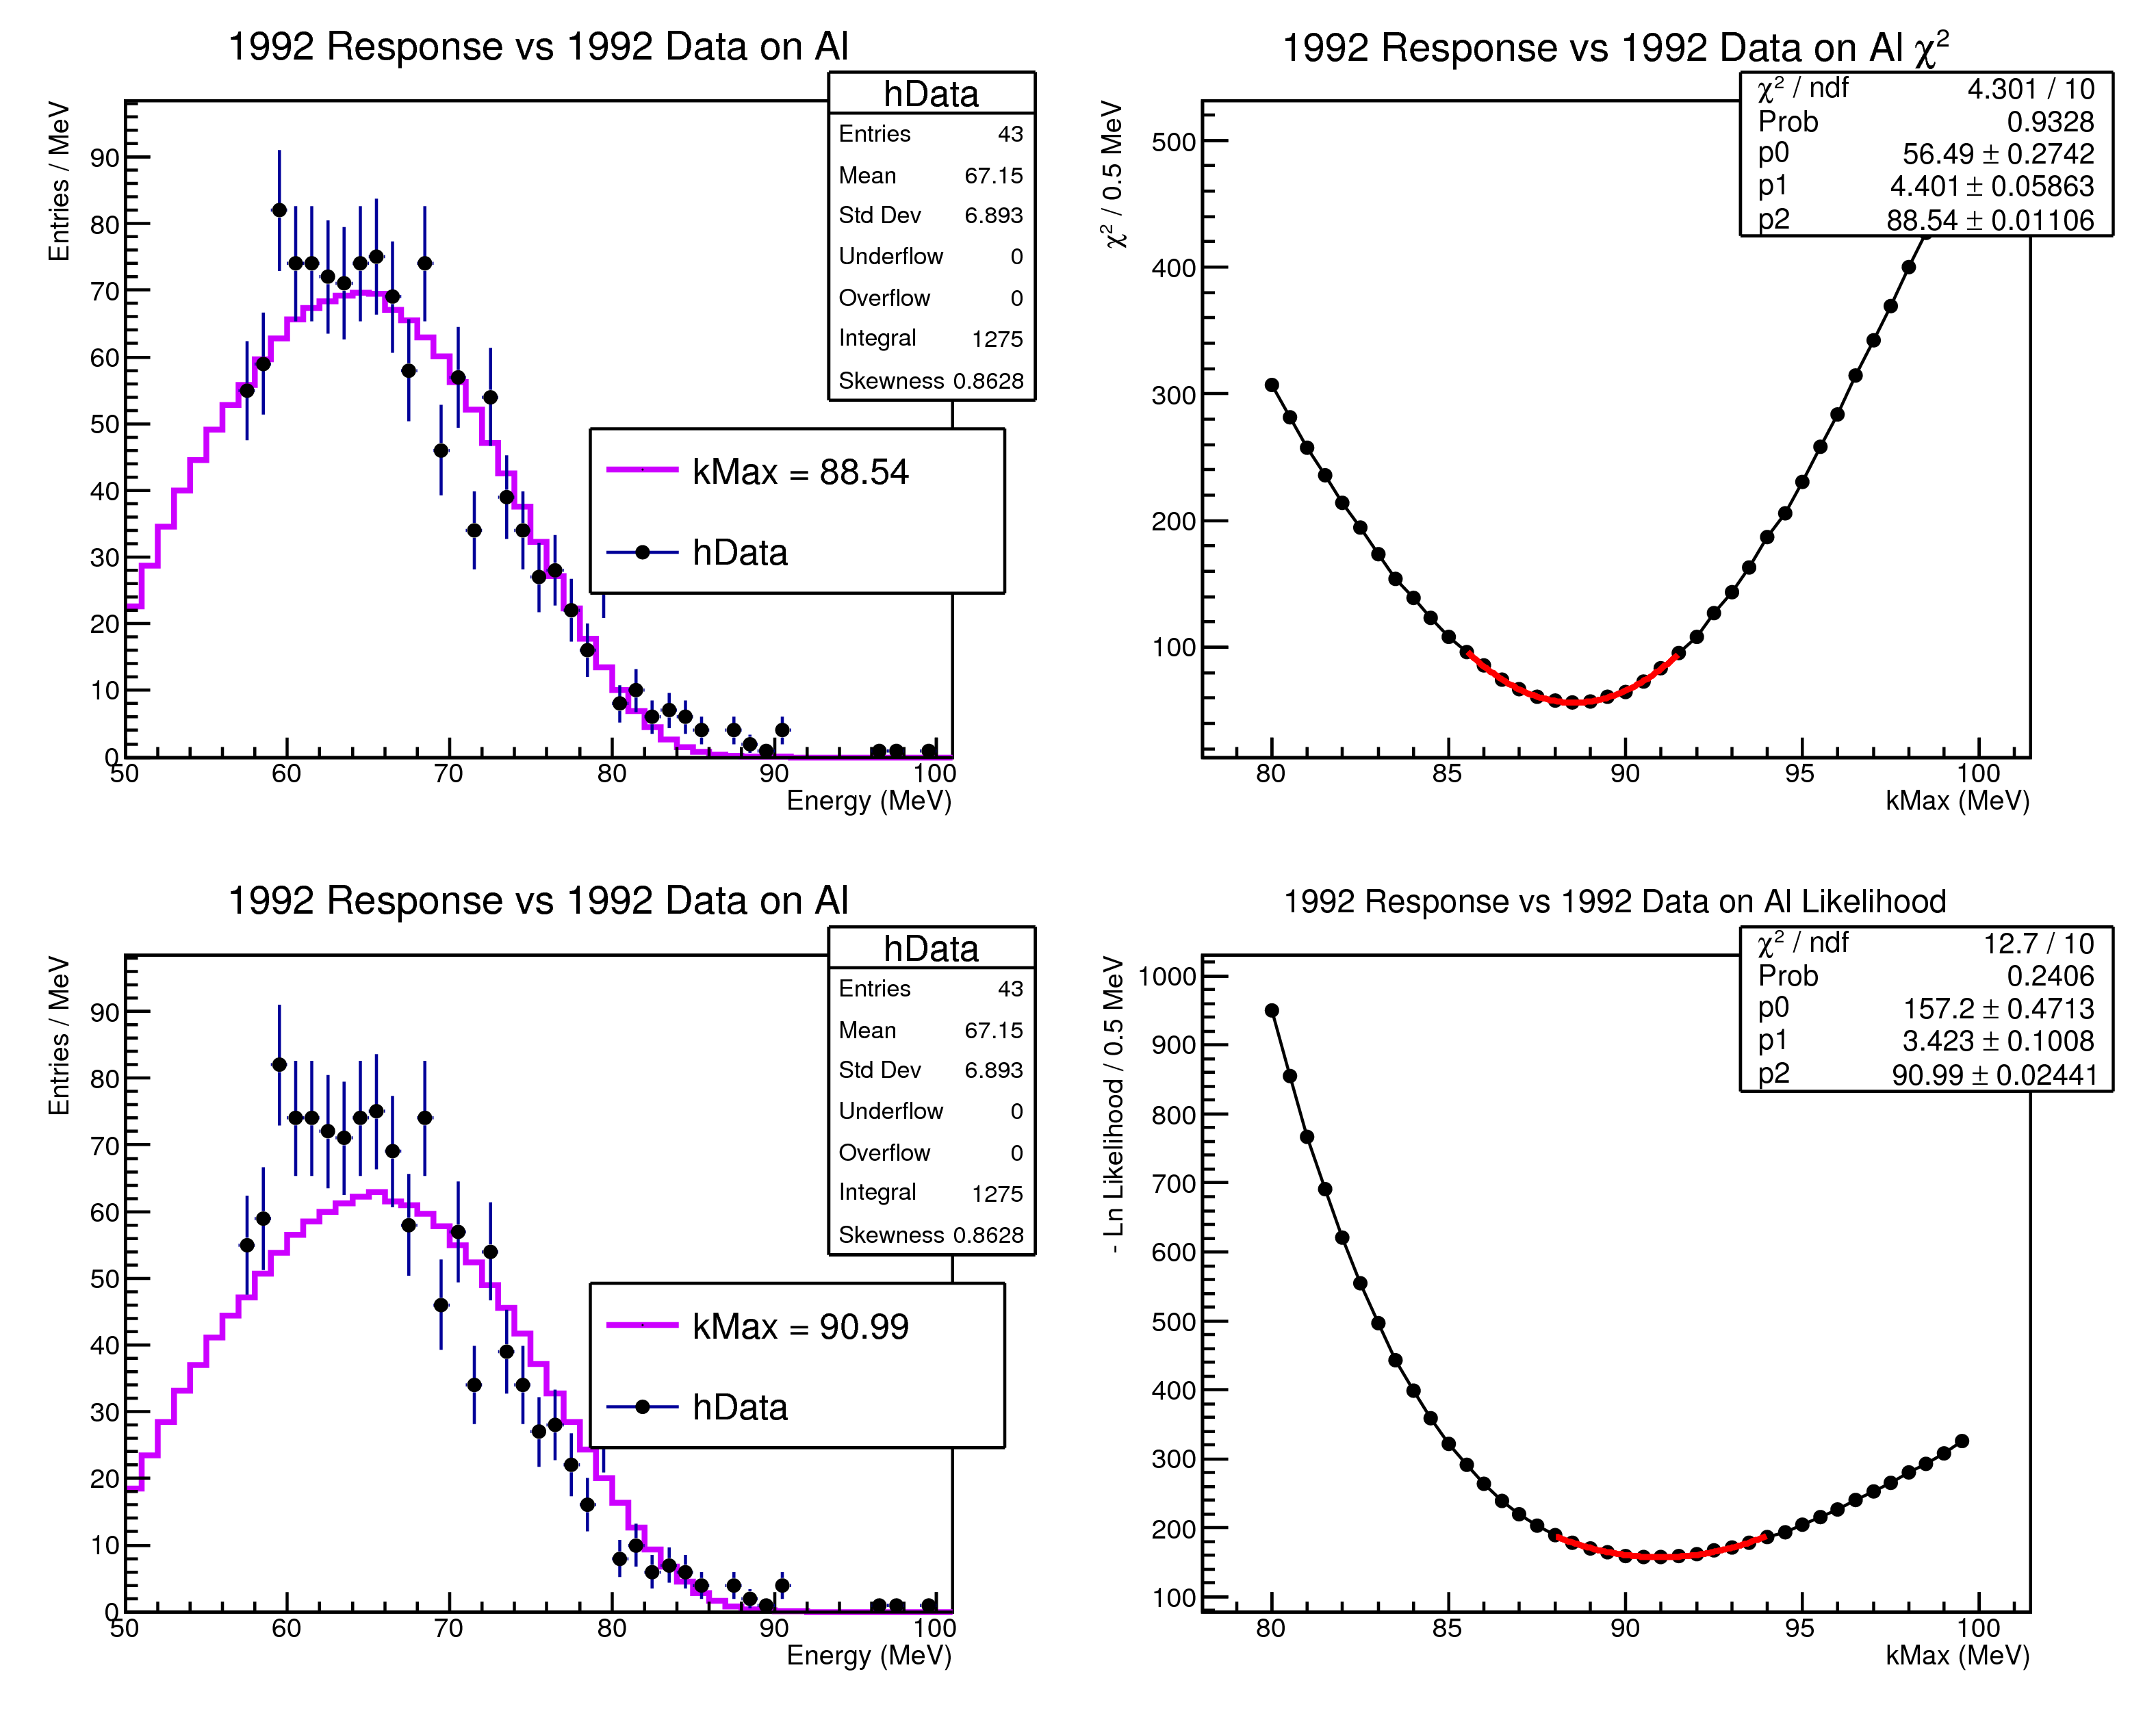
\includegraphics[width=0.8\linewidth]{figures/png/1992_resp_1992_Al_data_allPlots_singleK.png}
  \caption{The left figures show the best fit convolved closure approximation spectrum. The right figures
  show the parabolic fit to find the best fit endpoint value. The top figures use $\chi ^2$ 
  minimization while the bottom figures use $\mathcal{L}$ minimization.}
  \label{fig:1992AlFits}
\end{figure}


\begin{figure}[h]
  \centering
  \subfloat[ $\chi^2$ Minimization Fit \label{fig:ChiSq}]{%
  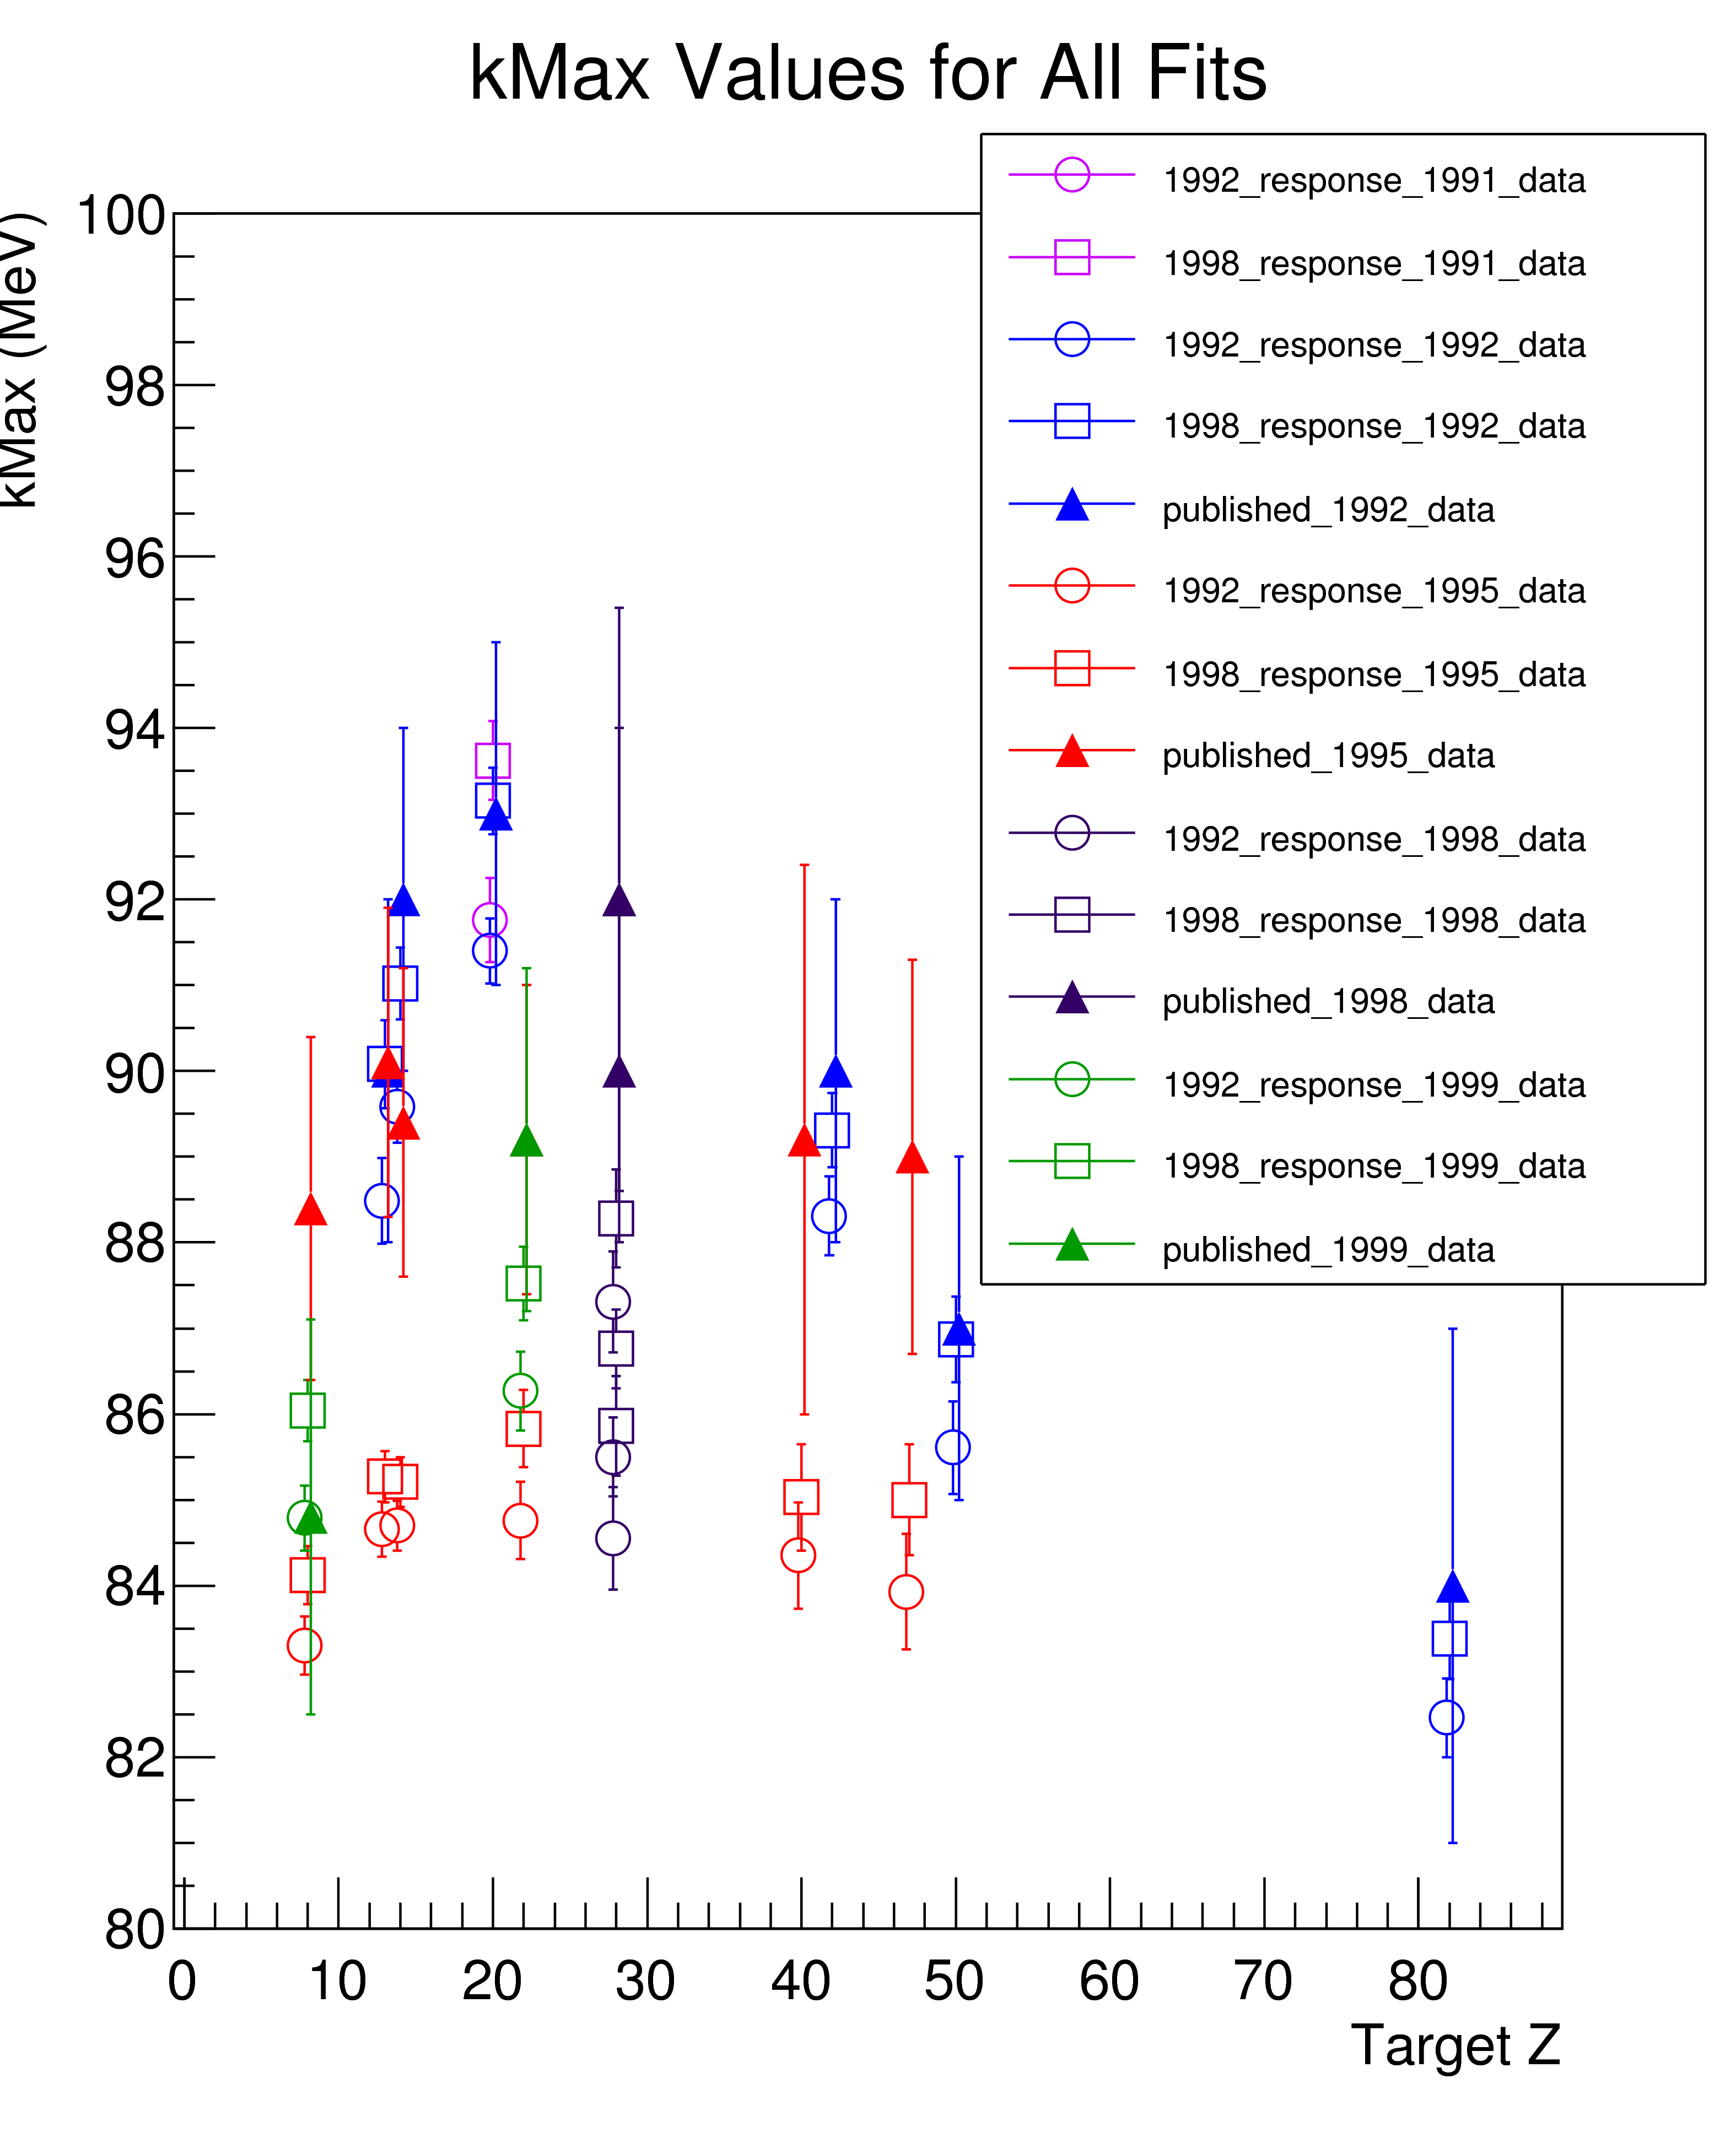
\includegraphics[width=0.48\linewidth]{figures/png/all_kMaxesChiSq_vs_target_z.png}
  }
  \hfill
  \subfloat[$\mathcal{L}$ Minimization Fit  \label{fig:NLL}]{%
  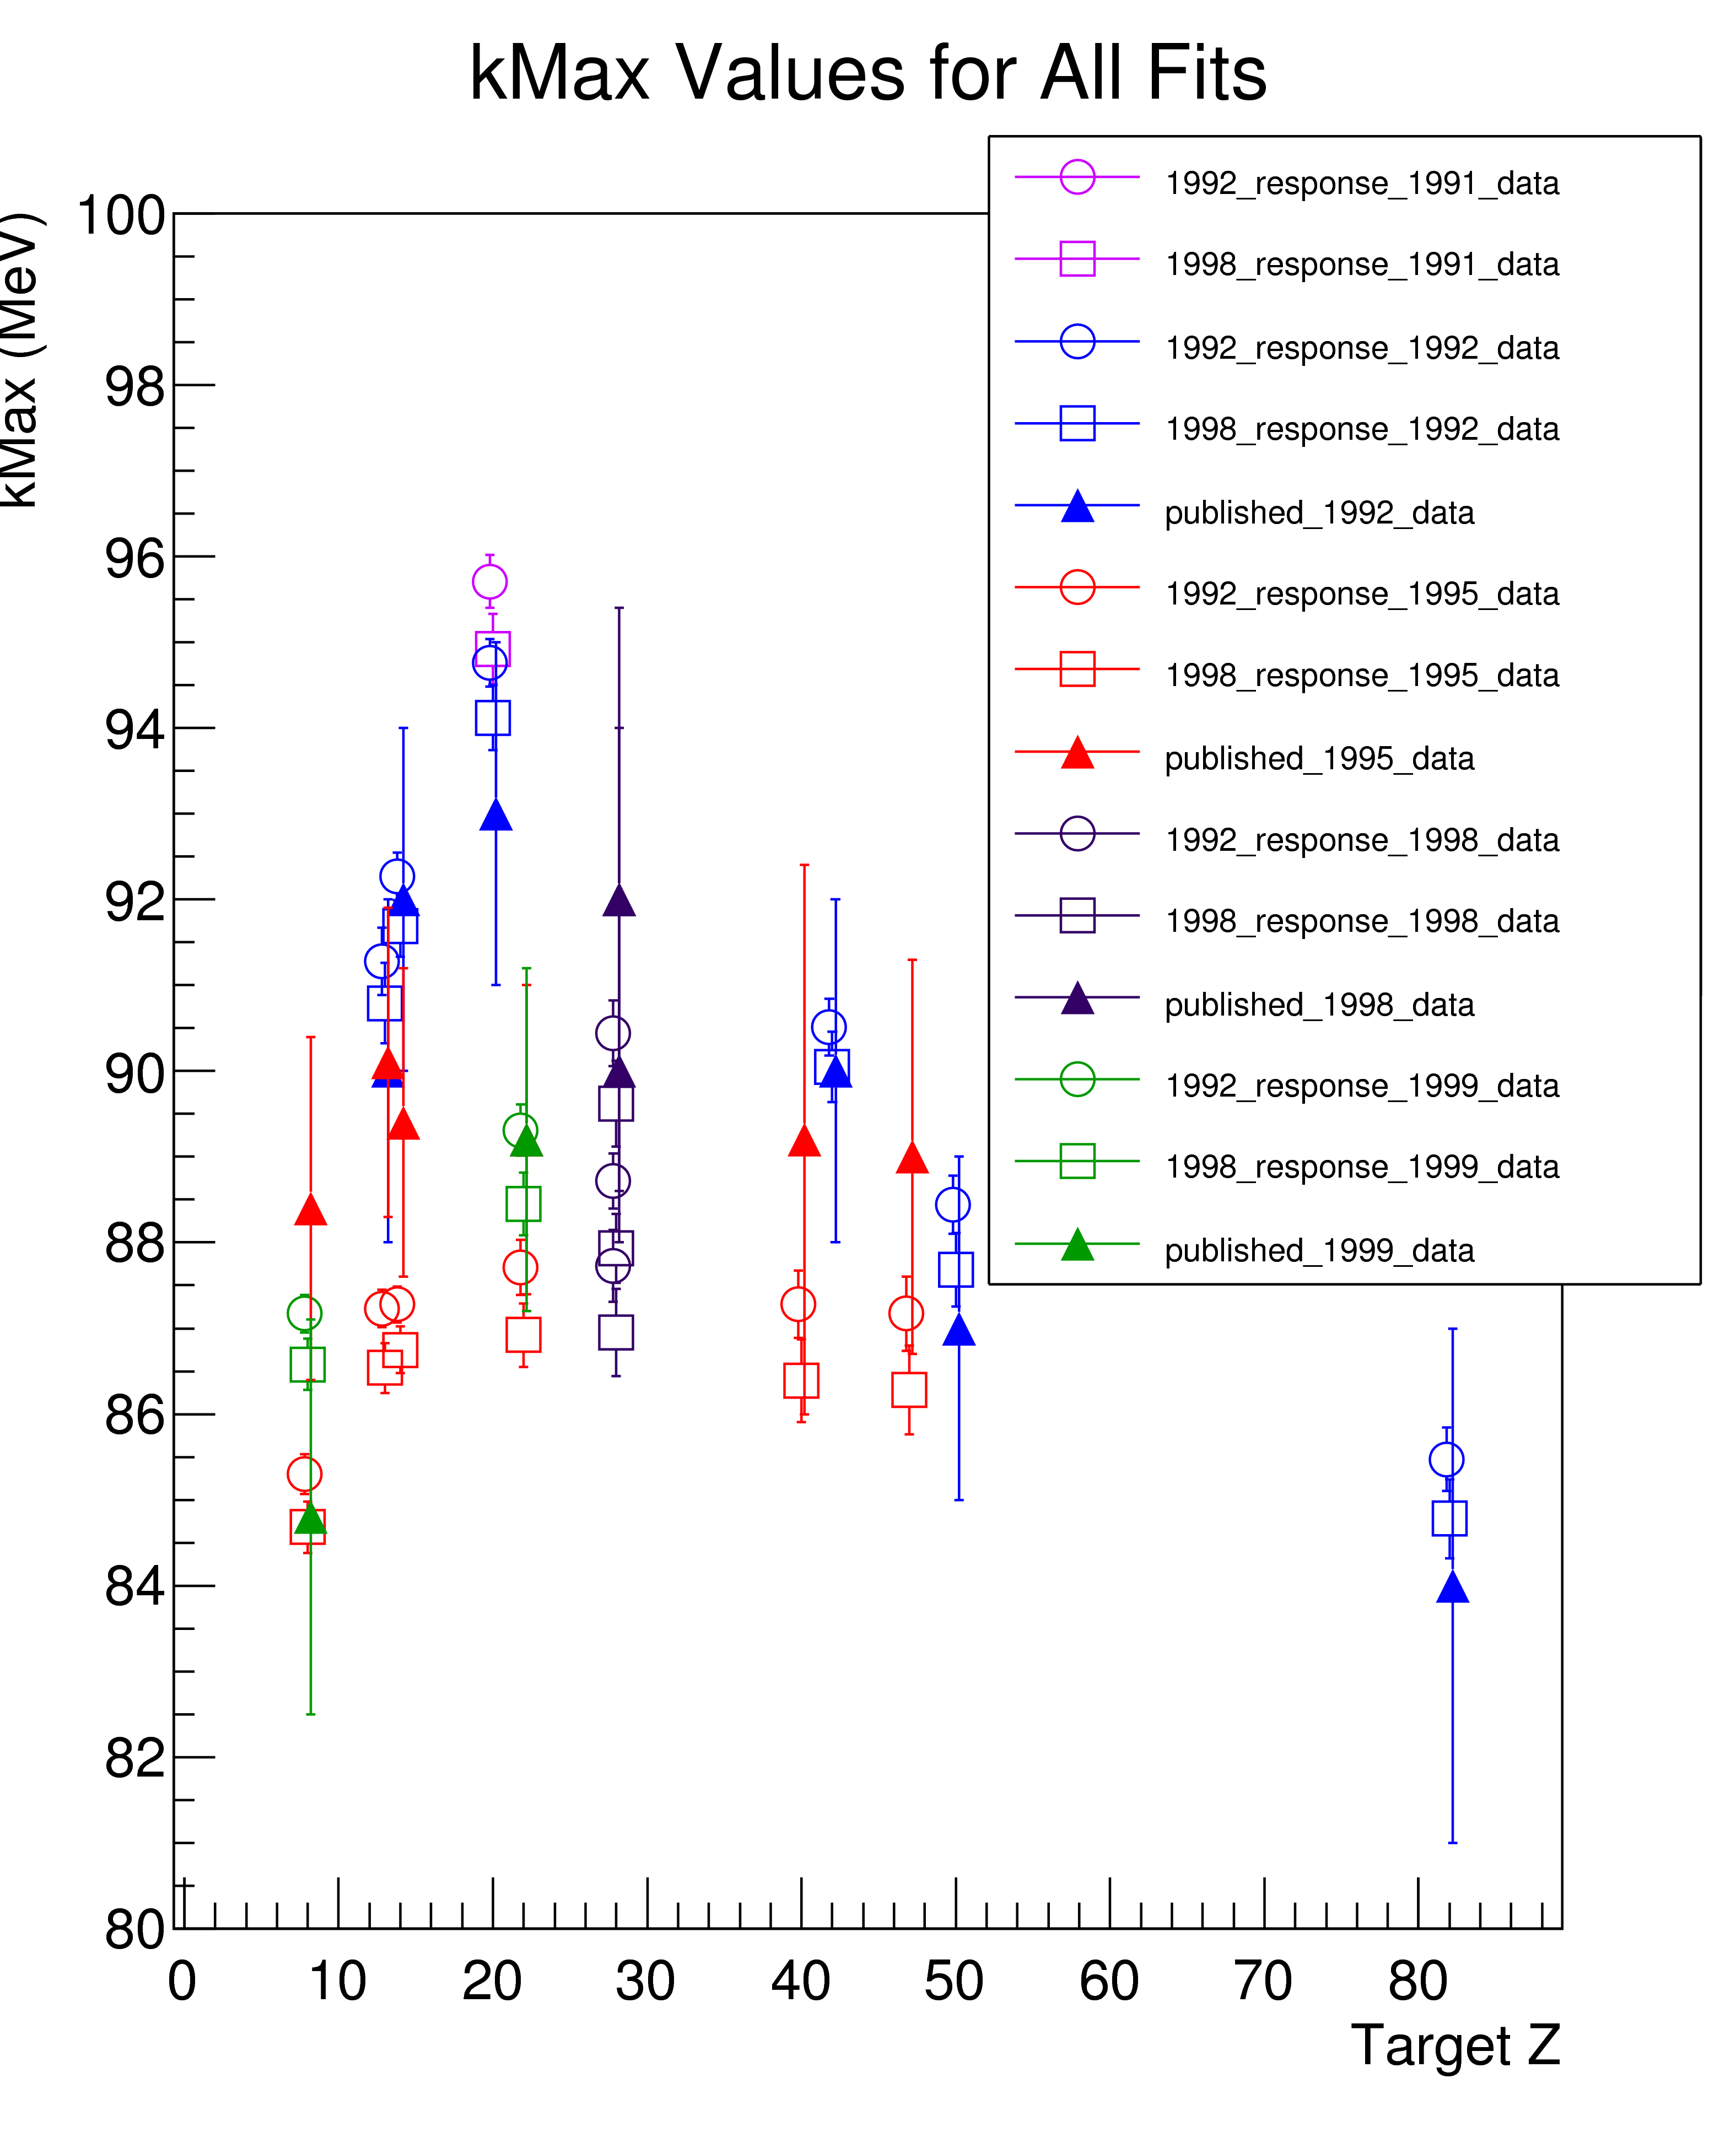
\includegraphics[width=0.48\linewidth]{figures/png/all_kMaxesNLL_vs_target_z.png}
  }
  \caption{Fit results vs target Z using (a) $\chi^2$ minimization and (b) $\mathcal{L}$ minimization.
    The 1992 detector response function data points (circles) are offset by -0.2 in z and the published data points (triangles)
    are offset by +0.2 in z.
  }
\end{figure}

\begin{figure}[h]
  \centering
  \includegraphics[width=0.8\linewidth]{figures/png/chiSq_of_fits.png}
  \caption{Fit $\chi^2$ values for both detector response functions and both fitting methods. }
  \label{fig:ChiSqOfFits}
\end{figure}

%% \begin{figure}[h]
%%   \centering
%%   \includegraphics[width=\linewidth]{figures/png/compare_fit_results.png}
%%   \caption{Plot of the difference between the end point values found using $\chi^2$ and
%%     $\mathcal{L}$ minimization with and without a restricted range using the 1998 detector response function.}
%%   \label{fig:compareFits}
%% \end{figure}

\begin{figure}[h]
  \centering
  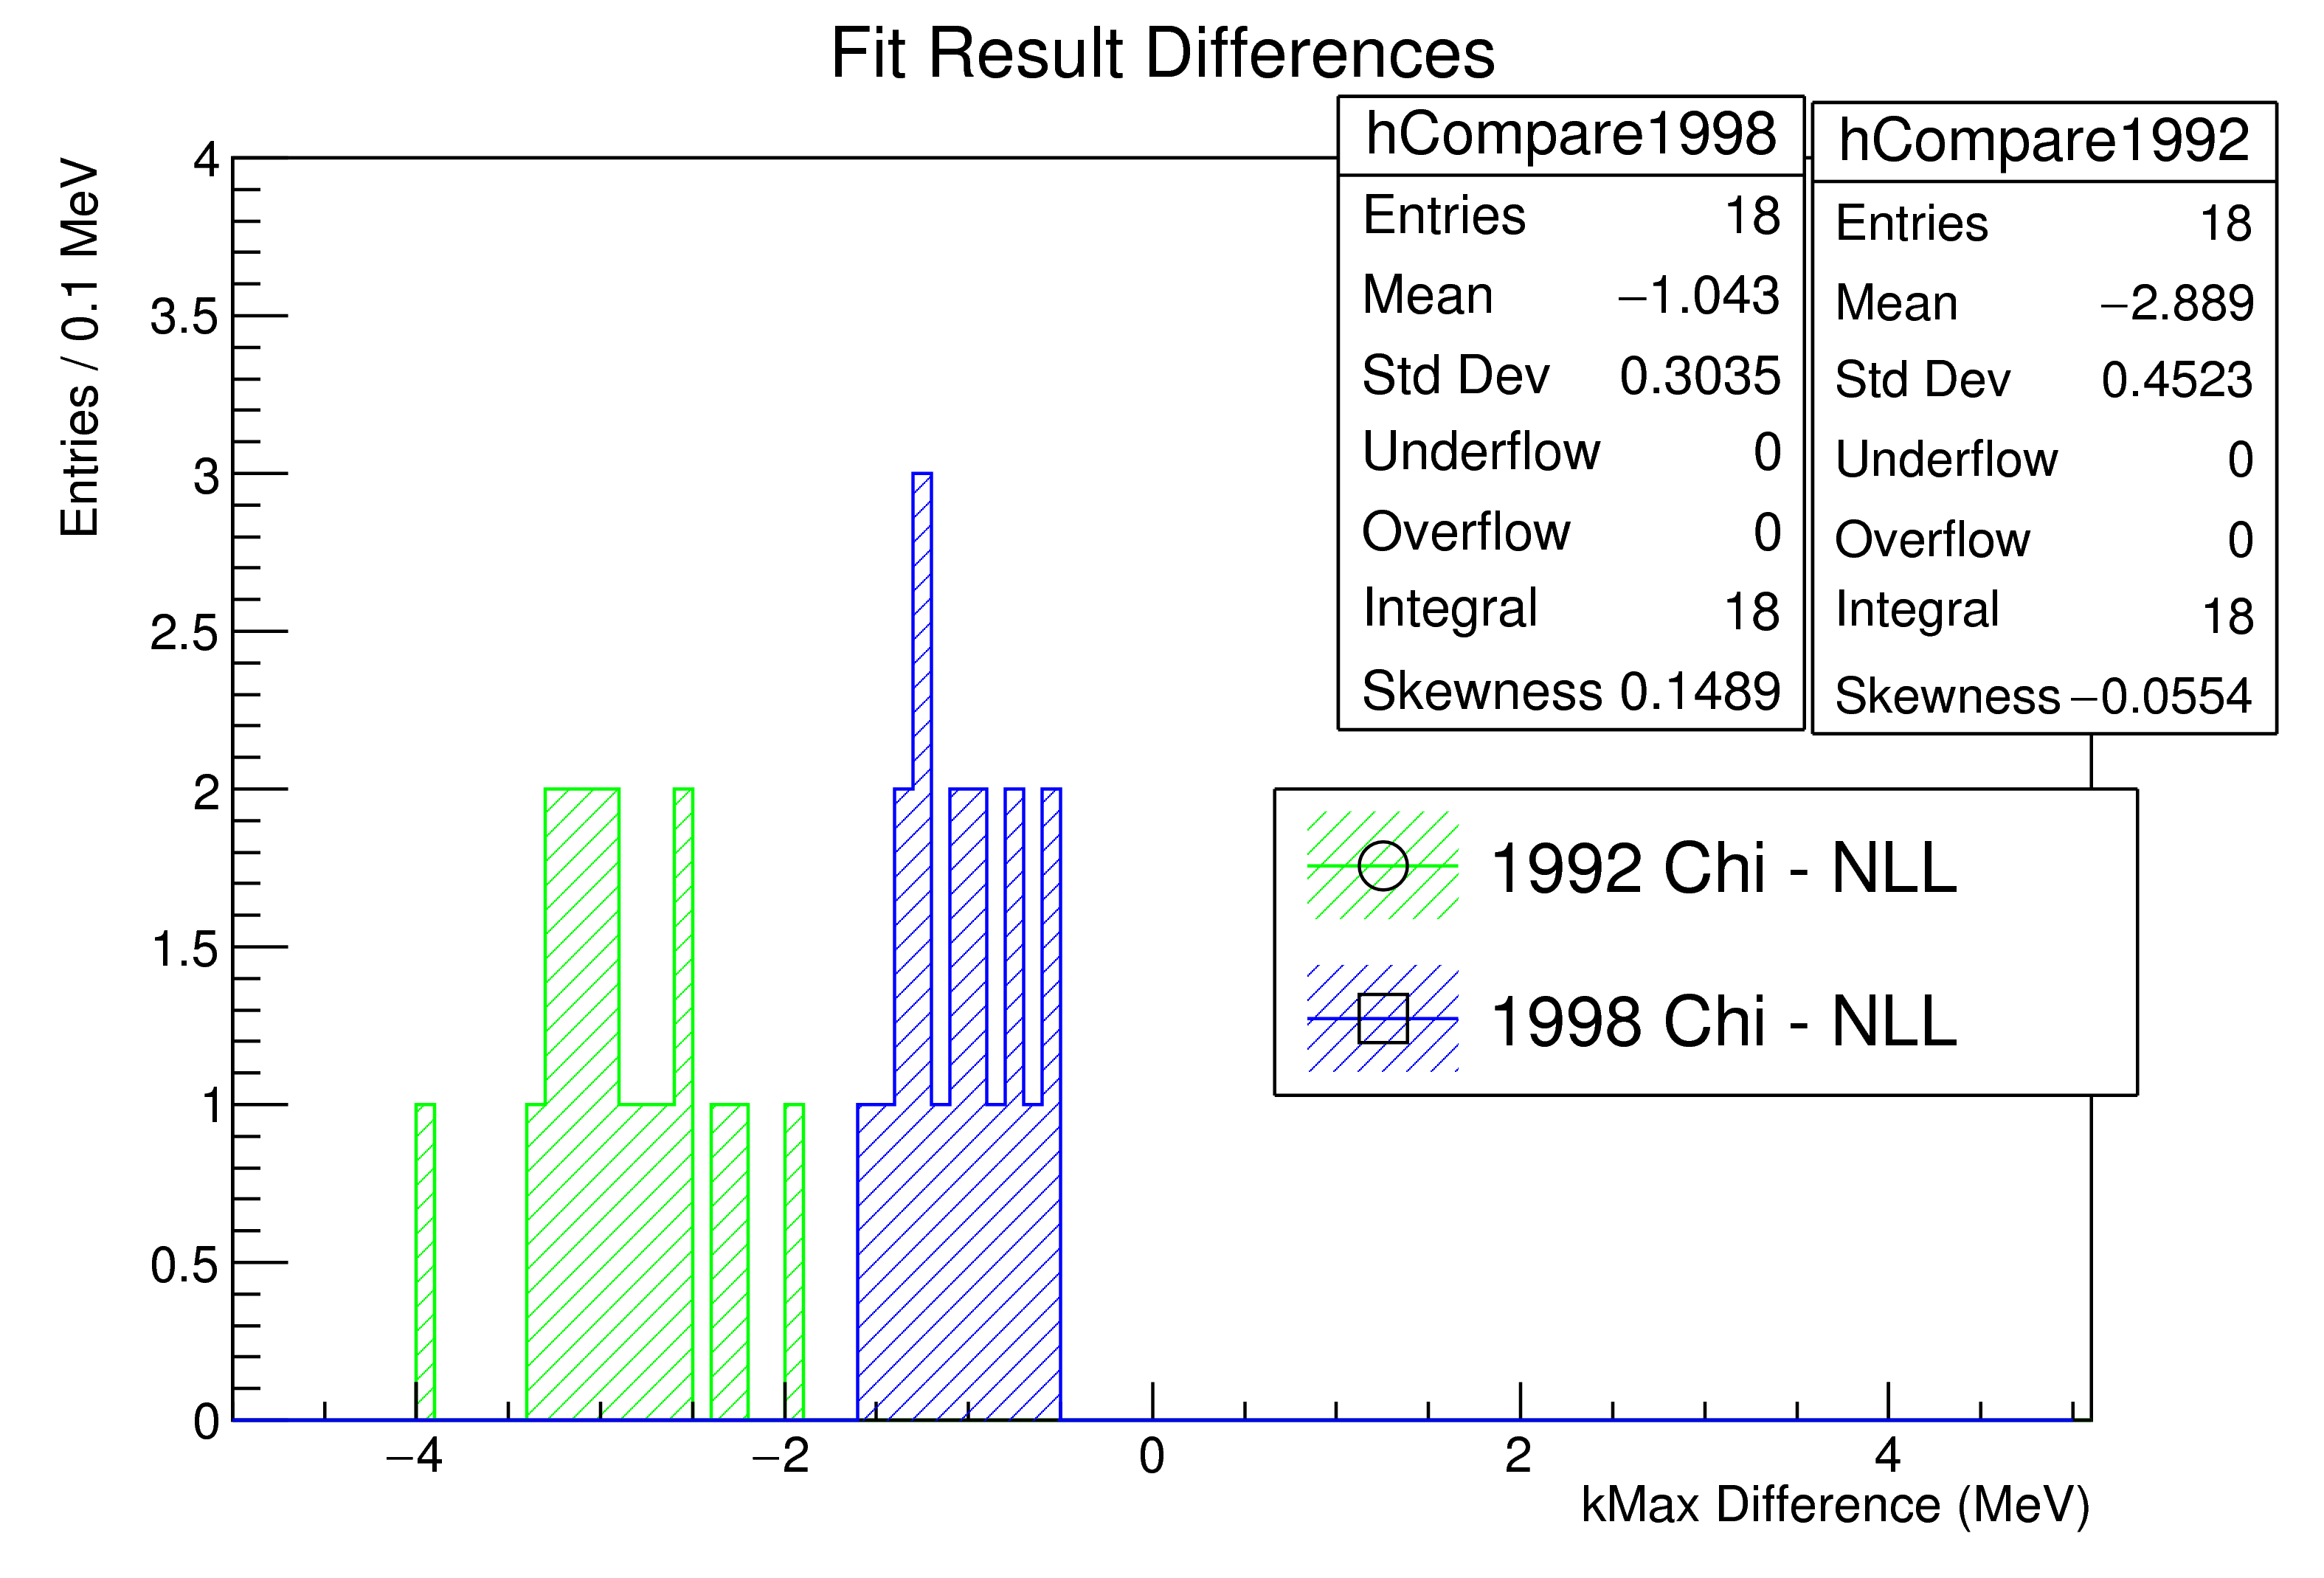
\includegraphics[width=\linewidth]{figures/png/compare_fit_results_92_v_98_unrestrictedOnly.png}
  \caption{Plot of the difference between the end point values found using $\chi^2$ and
    $\mathcal{L}$ minimization using the 1992 and 1998 detector response functions.}
  \label{fig:compareFits}
\end{figure}


\begin{figure}[h]
  \centering
  \subfloat[ 1992 detector response \label{fig:1992ToyErrs}]{%
  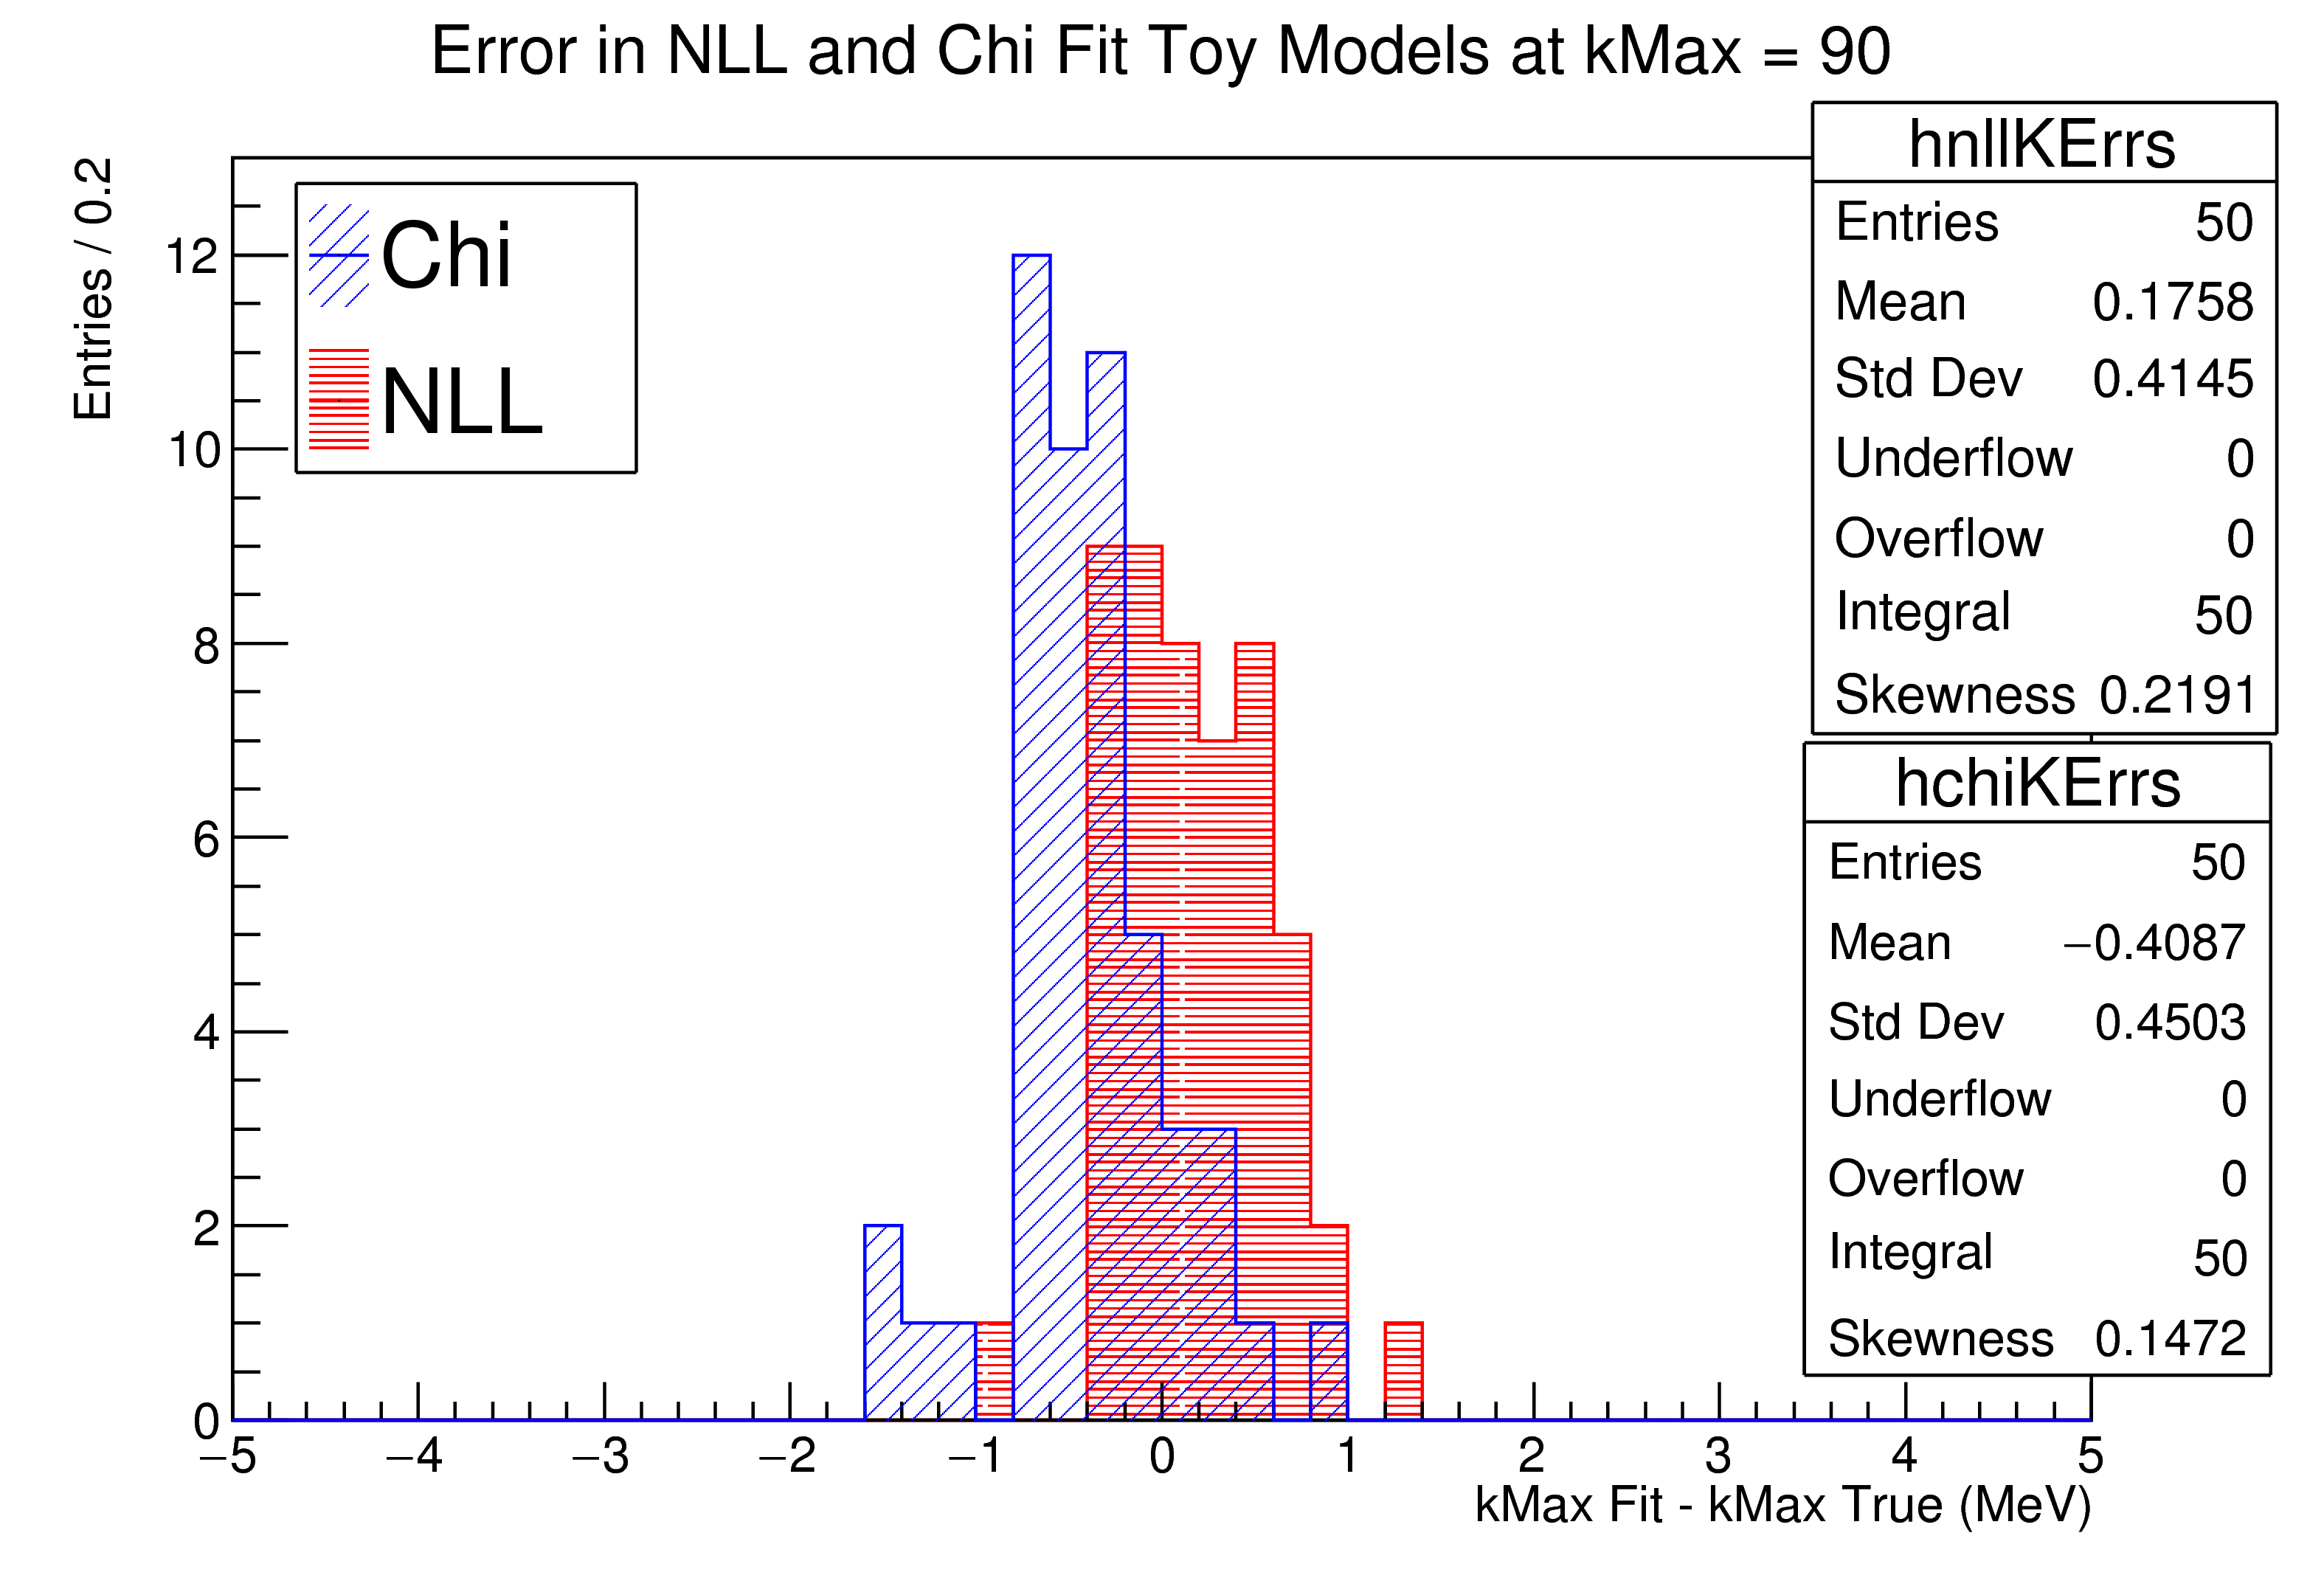
\includegraphics[width=0.48\linewidth]{figures/png/toy_kMax_errors_1992_response.png}
  }
  \hfill
  \subfloat[ 1998 detector response  \label{fig:1998ToyErrs}]{%
  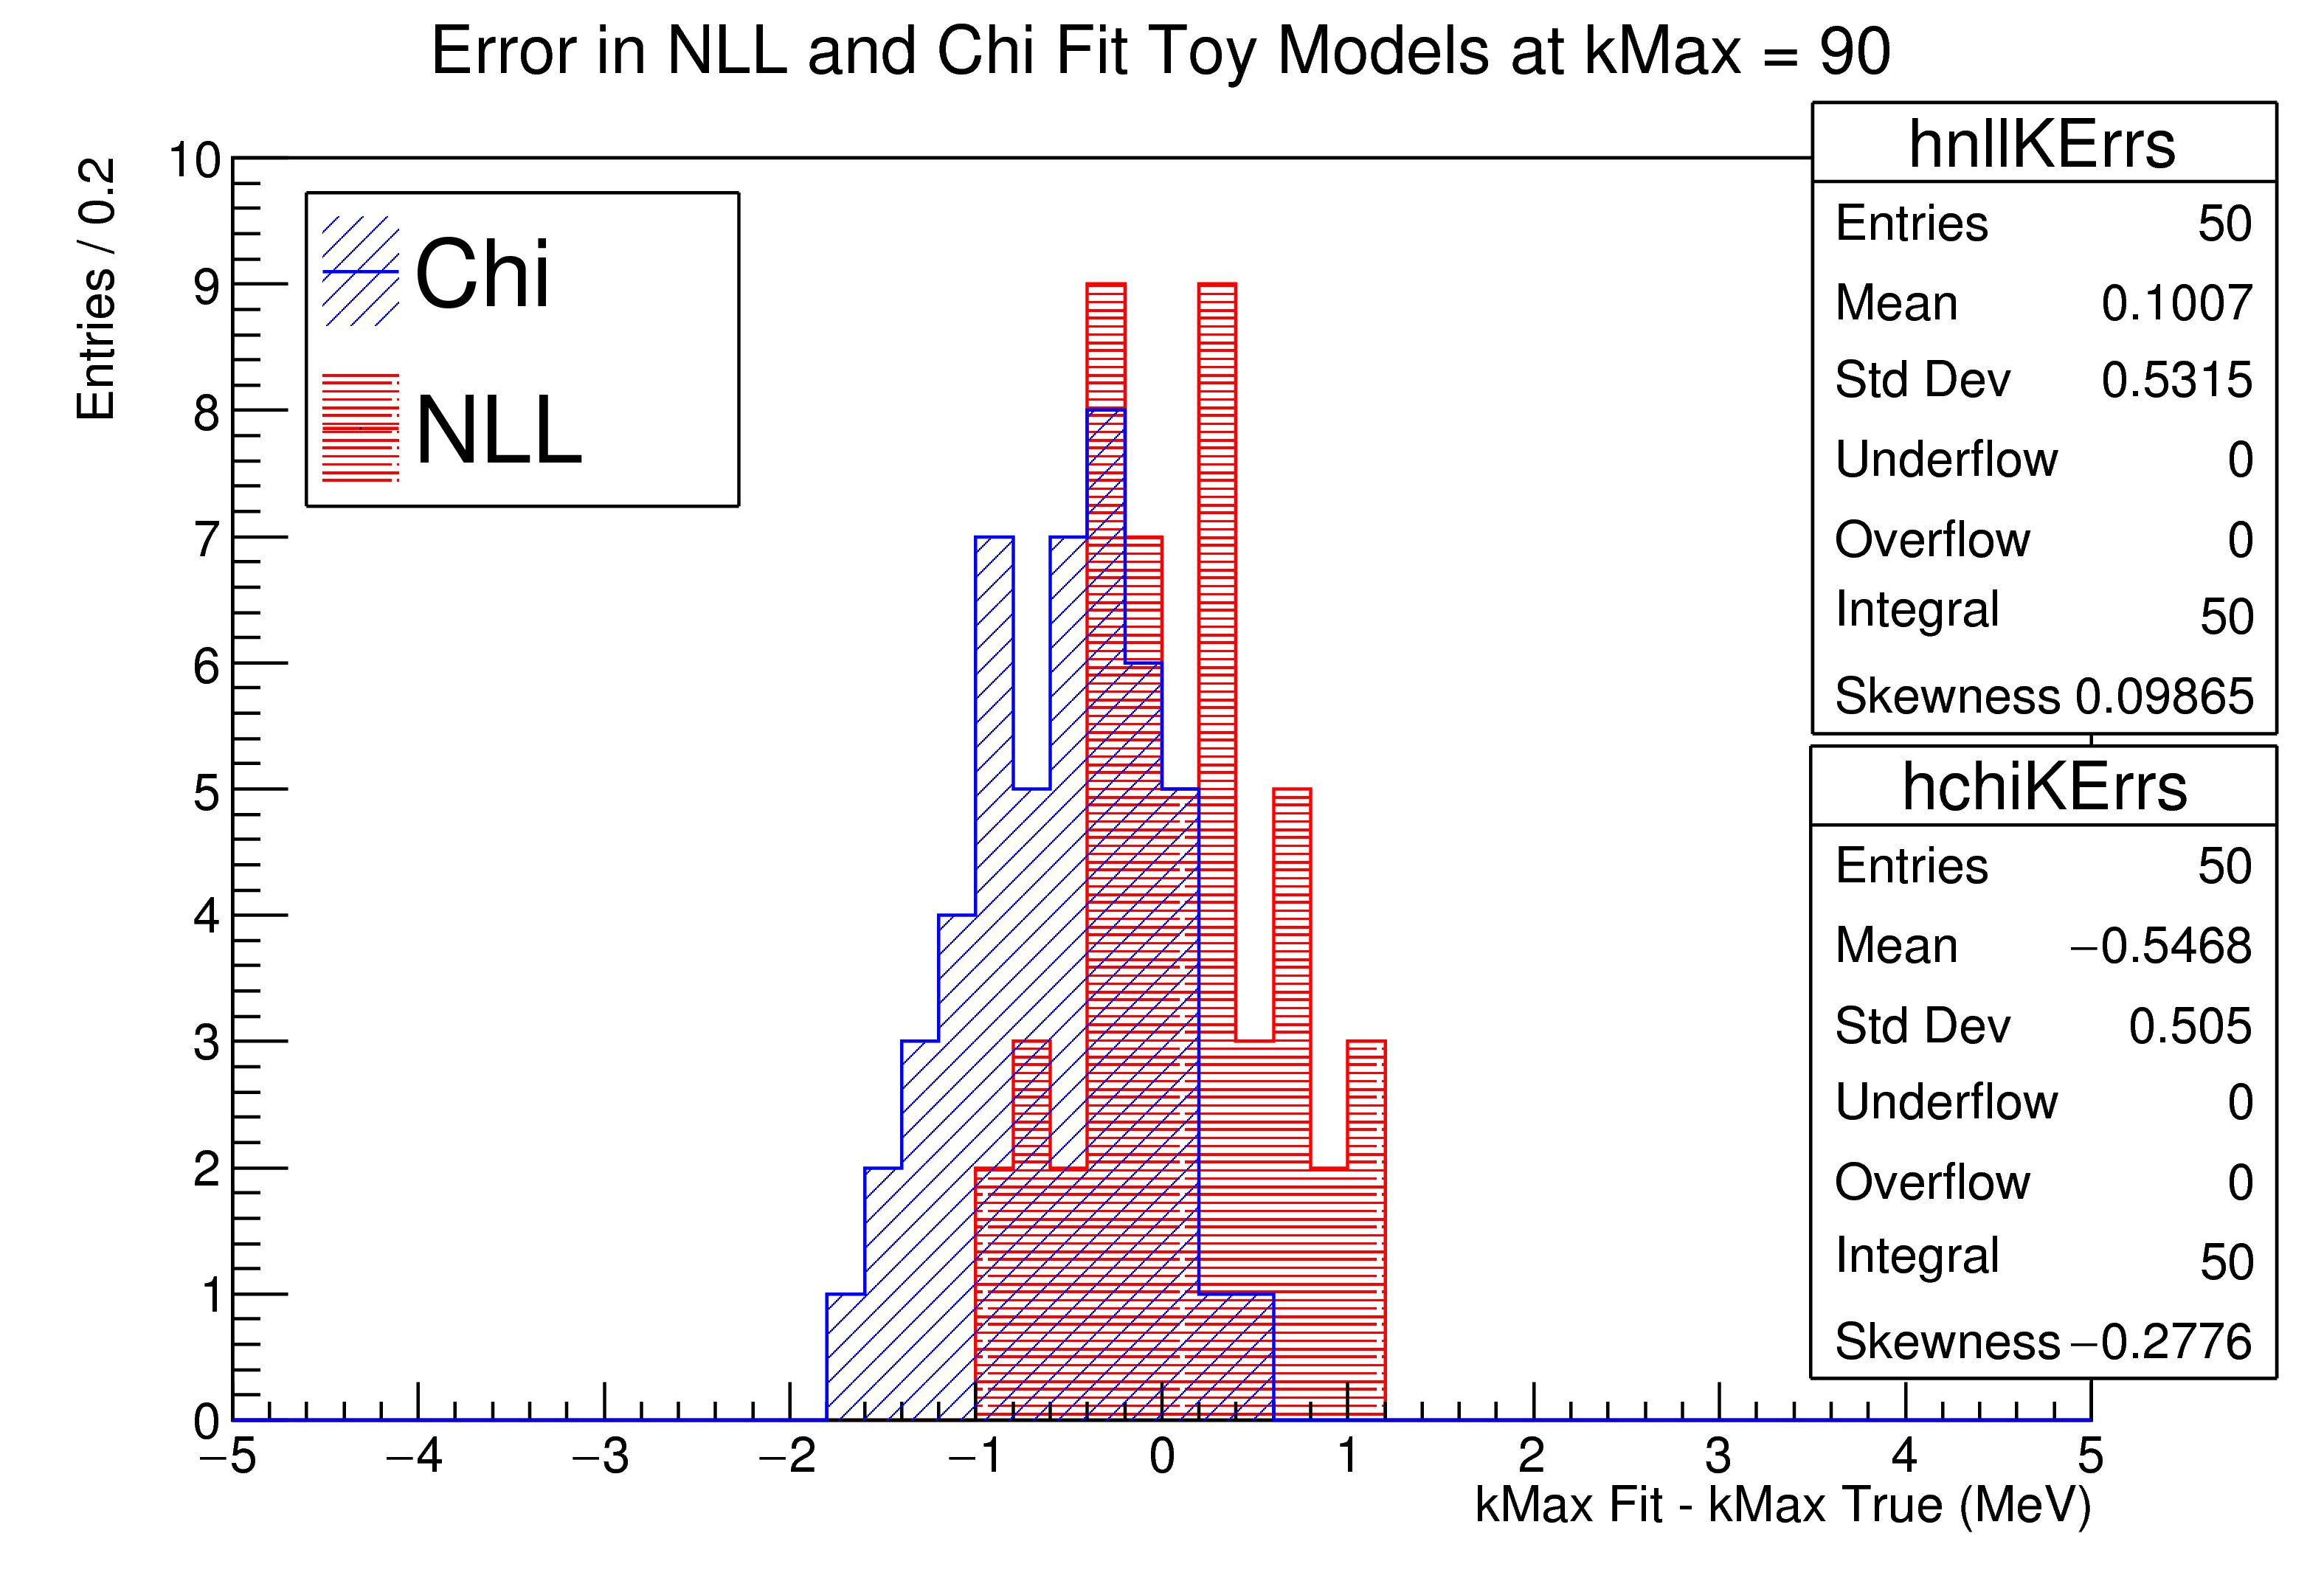
\includegraphics[width=0.48\linewidth]{figures/png/toy_kMax_errors_1998_response.png}
  }
  \caption{Fit results errors for 50 toy data sets using the (a) 1992 or (b) 1998 detector response function.
    The toy data sets are generated from a convolution with an end point value of 90 MeV and generated
    with 1275 data points.
  }
  \label{fig:ToyFitErrs}
\end{figure}


%% \begin{figure}[h]
%%   \centering
%%   \subfloat[ 1992 detector response \label{fig:1992ToyZs}]{%
%%   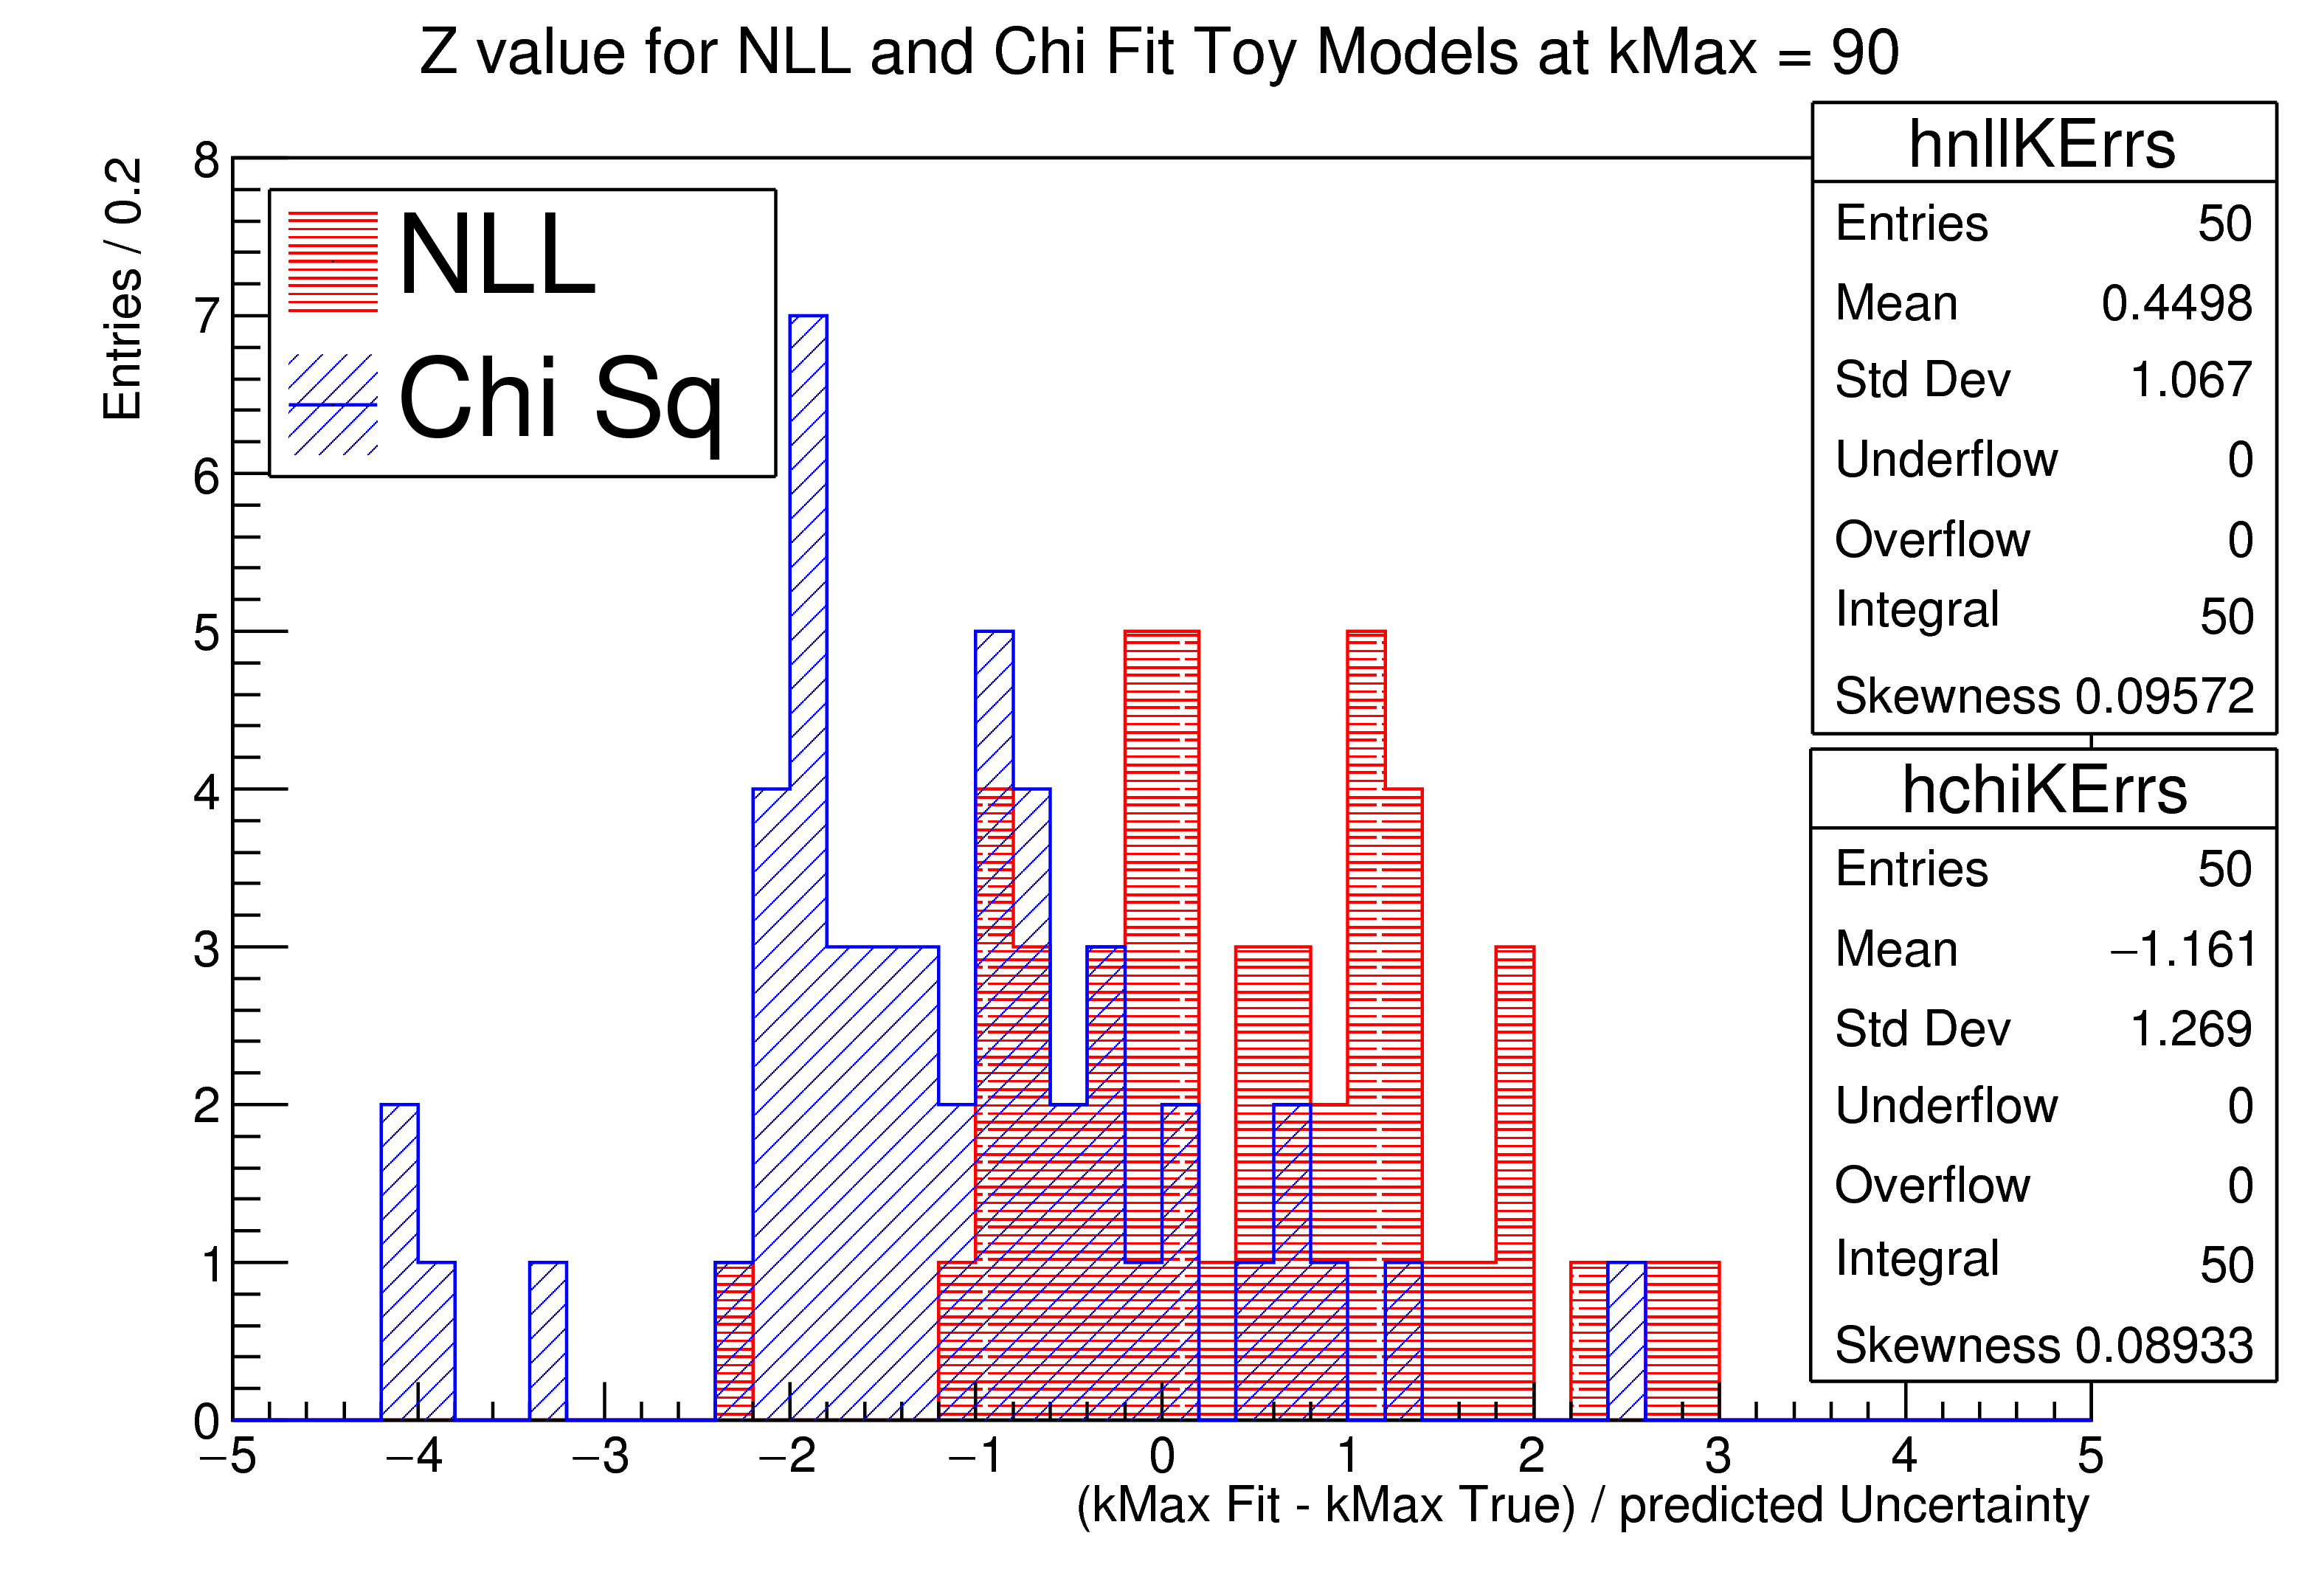
\includegraphics[width=0.48\linewidth]{figures/png/toy_kMax_z_values_1992_response.png}
%%   }
%%   \hfill
%%   \subfloat[ 1998 detector response  \label{fig:1998ToyZs}]{%
%%   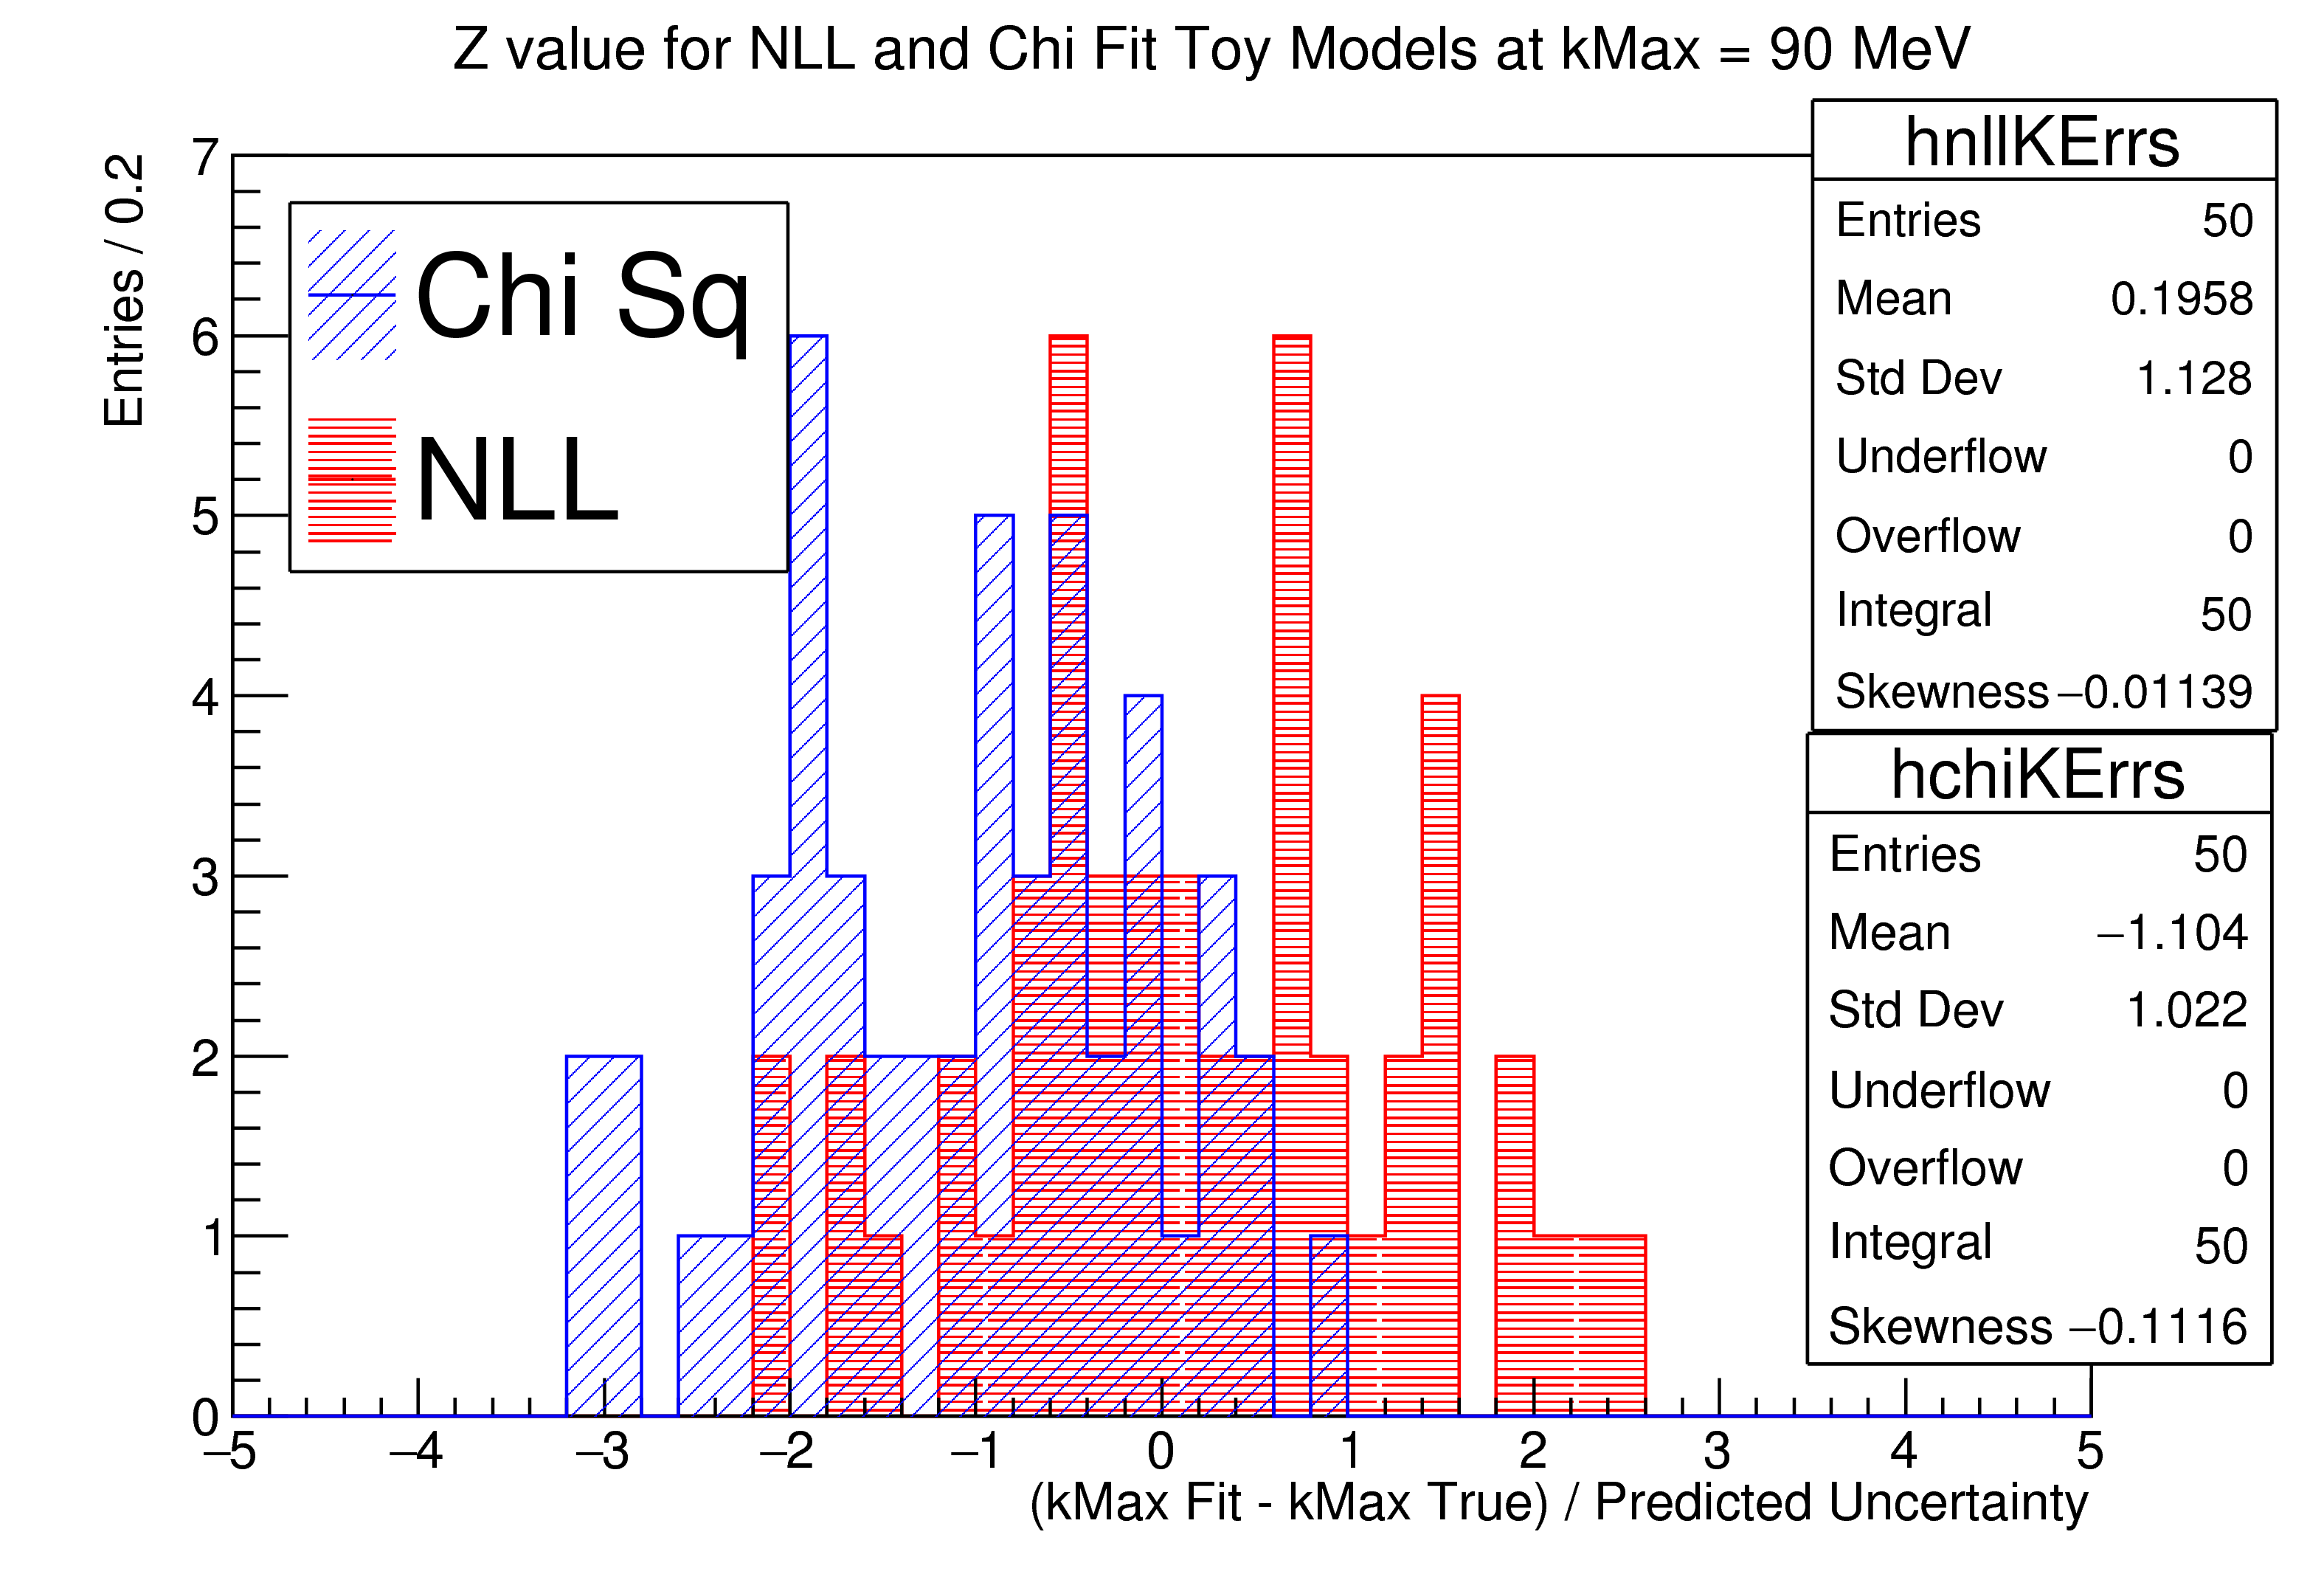
\includegraphics[width=0.48\linewidth]{figures/png/toy_kMax_z_values_1998_response.png}
%%   }
%%   \caption{Fit results z values for 50 toy data sets using the (a) 1992 or (b) 1998 detector response function.
%%     The toy data sets are generated from a convolution with an end point value of 90 MeV and generated
%%     with 1275 data points. The z value for a fit is the fit end point value minus the true value, divided
%%     by the fit estimated uncertainty. 
%%   }
%%   \label{fig:ToyFitZs}
%% \end{figure}



%%%%%%%%%%%%%%%%%%%%%%%%%%%%%%%%%%%%%%%%%%%%%%%%%%%%%%%%%%%%%%%%%%%%%%%%%%%%%%


\subsection { Fits of the 1992 data }
\begin{table}[h]
  \begin{center}
    \begin{tabular}{|l||l|l|l|l|l|l|}
      \hline
      Dataset & Published $k_{Max}$ & $\chi^2 / DoF$ & Our $k_{Max}$ & $\chi^2 / DoF$  & Response & Fit \\
      \hhline{|=||=|=|=|=|=|=|}
       Al 1992   & 90   $\pm$ 2   & 1.1 & 88.5 $\pm$ 0.5 &  1.6 (56.0 / 34) & 1992 & $\chi^2$ \\  
                 &                &     & 90.1 $\pm$ 0.5 &  1.2 (40.1 / 34) & 1998 & $\chi^2$ \\  
                                                                             
                 &                &     & 91.3 $\pm$ 0.4 & 2.3 ( 100.9 / 43)& 1992 & $\mathcal{L}$ \\
                 &                &     & 90.8 $\pm$ 0.5 & 1.5 ( 63.0 / 43) & 1998 & $\mathcal{L}$ \\
       \hline                                                                
       Ca 1992   & 93   $\pm$ 2   & 1.6 & 91.4 $\pm$ 0.4 &  2.6 (100.2 / 39)& 1992 & $\chi^2$ \\  
                 &                &     & 93.1 $\pm$ 0.4 &  1.4 (52.7 / 39) & 1998 & $\chi^2$ \\  
                                                                             
                 &                &     & 94.8 $\pm$ 0.3 & 4.6 ( 196.5 / 43)& 1992 & $\mathcal{L}$ \\
                 &                &     & 94.1 $\pm$ 0.4 & 1.7 ( 72.5 / 43) & 1998 & $\mathcal{L}$ \\
      \hline                                                                 
       Mo 1992   & 90   $\pm$ 2   & 0.8 & 88.3 $\pm$ 0.5 &  1.6 (50.3 / 32) & 1992 & $\chi^2$ \\  
                 &                &     & 89.3 $\pm$ 0.4 &  0.8 (24.7 / 32) & 1998 & $\chi^2$ \\  
                                                                             
                 &                &     & 90.1 $\pm$ 0.4 & 0.7 ( 29.2 / 43) & 1992 & $\mathcal{L}$ \\
                 &                &     & 90.5 $\pm$ 0.3 & 1.6 ( 70.9 / 43) & 1998 & $\mathcal{L}$ \\
      \hline                                                                 
       Pb 1992   & 84   $\pm$ 3   & 0.9 & 82.5 $\pm$ 0.5 &  1.3 (41.1 / 31) & 1992 & $\chi^2$ \\  
                 &                &     & 83.4 $\pm$ 0.5 &  0.6 (18.2 / 31) & 1998 & $\chi^2$ \\  
                                                                             
                 &                &     & 85.5 $\pm$ 0.4 & 2.1 ( 92.3 / 43) & 1992 & $\mathcal{L}$ \\
                 &                &     & 84.8 $\pm$ 0.5 & 0.7 ( 28.7 / 43) & 1998 & $\mathcal{L}$ \\
      \hline                                                                 
       Si 1992   & 92   $\pm$ 2   & 1.7 & 89.6 $\pm$ 0.4 &  3.1 (102.9 / 33)& 1992 & $\chi^2$ \\  
                 &                &     & 91.0 $\pm$ 0.4 &  1.3 (42.4 / 33) & 1998 & $\chi^2$ \\  
                                                                             
                 &                &     & 92.3 $\pm$ 0.3 & 3.4 ( 147.7 / 43)& 1992 & $\mathcal{L}$ \\
                 &                &     & 91.7 $\pm$ 0.4 & 1.2 ( 52.6 / 43) & 1998 & $\mathcal{L}$ \\
      \hline                                                                 
       Sn 1992   & 87   $\pm$ 2   & 1.1 & 85.6 $\pm$ 0.5 &  2.4 (74.7 / 31) & 1992 & $\chi^2$ \\  
                 &                &     & 86.9 $\pm$ 0.5 &  0.7 (21.7 / 31) & 1998 & $\chi^2$ \\  
                                                                             
                 &                &     & 88.4 $\pm$ 0.3 & 2.5 ( 109.6 / 43) & 1992 & $\mathcal{L}$ \\
                 &                &     & 87.7 $\pm$ 0.4 & 0.6 ( 26.6 / 43) & 1998 & $\mathcal{L}$ \\
      \hline                           
    \end{tabular}
  \end{center}
  \caption{The fit results.}
  \label{table:fits1992}
\end{table}

%%%%%%%%%%%%%%%%%%%%%%%%%%%%%%%%%%%%%%%%%%%%%%%%%%%%%%%%%%%%%%%%%%%%%%%%%%%%%%
\subsection { Fits of the 1995 data }

\begin{table}[h]
  \begin{center}
    \begin{tabular}{|l||l|l|l|l|l|l|}
      \hline
      Dataset & Published $k_{Max}$ & $\chi^2 / DoF$ & Our $k_{Max}$ & $\chi^2 / DoF$  & Response & Fit \\
      \hhline{|=||=|=|=|=|=|=|}
       Ag 1995   & 89.0 $\pm$ 3.2 & 1.2 &83.9 $\pm$ 0.7 &  2.0 (60.7 / 30)  & 1992 & $\chi^2$ \\  
                 &                &     &85.0 $\pm$ 0.7 &  1.0 (29.2 / 30)  & 1998 & $\chi^2$ \\  
                                                                             
                &                &     & 87.2 $\pm$ 0.4 & 2.2 ( 93.8 / 43) & 1992 & $\mathcal{L}$ \\
                &                &     & 86.3 $\pm$ 0.5 & 0.8 ( 35.9 / 43) & 1998 & $\mathcal{L}$ \\      
      \hline                                                                
       Al 1995   & 90.1 $\pm$ 1.8 & 1.5 &84.7 $\pm$ 0.3 &  4.2 (134.9 / 32) & 1992 & $\chi^2$ \\  
                 &                &     &85.3 $\pm$ 0.3 &  1.3 (41.9 / 32)  & 1998 & $\chi^2$ \\  
                                                                            
                &                &     & 87.2 $\pm$ 0.2 & 4.7 ( 203.1 / 43) & 1992 & $\mathcal{L}$ \\
                &                &     & 86.5 $\pm$ 0.3 & 1.3 ( 54.3 / 43) & 1998 & $\mathcal{L}$ \\
      \hline                                                                
       O 1995    & 88.4 $\pm$ 2.3 & 2.1 &83.3 $\pm$ 0.3 &  4.5 (113.5 / 25) & 1992 & $\chi^2$ \\  
                 &                &     &84.1 $\pm$ 0.3 &  1.3 (33.3 / 25)  & 1998 & $\chi^2$ \\  
                                                                            
                &                &     & 85.3 $\pm$ 0.2 & 3.6 ( 153.5 / 43)& 1992 & $\mathcal{L}$\\
                &                &     & 84.7 $\pm$ 0.3 & 1.1 ( 48.3 / 43) & 1998 & $\mathcal{L}$\\
      \hline                                                                     
       Si 1995   & 89.4 $\pm$ 1.8 & 2.7 &84.7 $\pm$ 0.3 &  4.9 (151.5 / 31) & 1992 & $\chi^2$ \\  
                 &                &     &85.2 $\pm$ 0.3 &  2.3 (71.9 / 31)  & 1998 & $\chi^2$ \\  
                                                                             
                &                &     & 87.3 $\pm$ 0.2 & 5.6 ( 241.5 / 43) & 1992 & $\mathcal{L}$ \\
                &                &     & 86.7 $\pm$ 0.3 & 2.4 ( 102.9 / 43)& 1998 & $\mathcal{L}$ \\
      \hline                                                                
       Ti 1995   & 89.2 $\pm$ 2.0 & 1.9 &84.8 $\pm$ 0.5 &  3.6 (116.0 / 32) & 1992 & $\chi^2$ \\  
                 &                &     &85.8 $\pm$ 0.4 &  1.5 (46.9 / 32)  & 1998 & $\chi^2$ \\  
                                                                            
                &                &     & 87.7 $\pm$ 0.3 & 3.9 ( 169.7 / 43) & 1992 & $\mathcal{L}$ \\
                &                &     & 86.9 $\pm$ 0.4 & 1.3 ( 57.4 / 43) & 1998 & $\mathcal{L}$ \\
      \hline                                                                
       Zr 1995   & 89.2 $\pm$ 3.4 & 1.2 &84.3 $\pm$ 0.6 &  2.9 (89.7 / 31)  & 1992 & $\chi^2$ \\  
                 &                &     &85.0 $\pm$ 0.6 &  1.6 (49.6 / 31)  & 1998 & $\chi^2$ \\  
                                                                            
                &                &     & 87.3 $\pm$ 0.4 & 2.9 ( 122.6 / 43) & 1992 & $\mathcal{L}$ \\
                &                &     & 86.4 $\pm$ 0.5 & 1.4 ( 59.4 / 43) & 1998 & $\mathcal{L}$ \\
      \hline
                                                                                
    \end{tabular}
  \end{center}
  \caption{The fit results.}
  \label{table:fits1995}
\end{table}


%%%%%%%%%%%%%%%%%%%%%%%%%%%%%%%%%%%%%%%%%%%%%%%%%%%%%%%%%%%%%%%%%%%%%%%%%%%%%%
\subsection { Fits of the 1998 data }
\begin{table}[h]
  \begin{center}
    \begin{tabular}{|l||l|l|l|l|l|l|}
      \hline
      Dataset & Published $k_{Max}$ & $\chi^2 / DoF$ & Our $k_{Max}$ & $\chi^2 / DoF$  & Response & Fit \\
      \hhline{|=||=|=|=|=|=|=|}
       Ni58 1998 & 92   $\pm$ 2   & 1.8 & 87.3 $\pm$ 0.6 &  2.3 (73.7 / 32) & 1992 & $\chi^2$ \\  
                 &                &     & 88.3 $\pm$ 0.6 &  1.0 (32.7 / 32) & 1998 & $\chi^2$ \\  
                                                                             
                &                 &     & 90.4 $\pm$ 0.4 & 2.5 ( 107.2 / 43) & 1992 & $\mathcal{L}$ \\
                &                 &     & 89.6 $\pm$ 0.5 & 0.9 ( 40.0 / 43) & 1998 & $\mathcal{L}$ \\
      \hline                                                                 
       Ni60 1998 & 92   $\pm$ 2   & 2.0 & 85.5 $\pm$ 0.5 &  2.6 (84.4 / 33) & 1992 & $\chi^2$ \\  
                 &                &     & 86.8 $\pm$ 0.5 &  1.1 (36.4 / 33) & 1998 & $\chi^2$ \\  
                                                                             
                &                 &     & 88.7 $\pm$ 0.3 & 3.5 ( 151.1 / 43) & 1992 & $\mathcal{L}$ \\
                &                 &     & 87.9 $\pm$ 0.4 & 1.1 ( 47.5 / 43) & 1998 & $\mathcal{L}$ \\
      \hline                                                                 
       Ni62 1998 & 90   $\pm$ 2   & 1.3 & 84.6 $\pm$ 0.6 &  1.7 (51.1 / 30) & 1992 & $\chi^2$ \\  
                 &                &     & 85.9 $\pm$ 0.6 &  0.8 (25.1 / 30) & 1998 & $\chi^2$ \\  
                                                                             
                &                 &     & 87.7 $\pm$ 0.4 & 2.1 ( 89.2 / 43) & 1992 & $\mathcal{L}$ \\
                &                 &     & 87.0 $\pm$ 0.5 & 0.7 ( 30.9 / 43) & 1998 & $\mathcal{L}$ \\
      \hline                           
    \end{tabular}
  \end{center}
  \caption{The fit results.}
  \label{table:fits1998}
\end{table}

%%%%%%%%%%%%%%%%%%%%%%%%%%%%%%%%%%%%%%%%%%%%%%%%%%%%%%%%%%%%%%%%%%%%%%%%%%%%%%
\subsection { Fits of the 1999 data }

\begin{table}[h]
  \begin{center}
    \begin{tabular}{|l||l|l|l|l|l|l|}
      \hline
      Dataset & Published $k_{Max}$ & $\chi^2 / DoF$ & Our $k_{Max}$ & $\chi^2 / DoF$  & Response & Fit \\
      \hhline{|=||=|=|=|=|=|=|}
       O 1999    & 88.4 $\pm$ 2.3 & 2.1 & 84.8 $\pm$ 0.4 &  5.6 (157.1 / 28)& 1992 & $\chi^2$ \\  
                 &                &     & 86.0 $\pm$ 0.4 &  1.7 (46.7 / 28) & 1998 & $\chi^2$ \\  
                                                                             
                 &                &     & 87.2 $\pm$ 0.2 & 5.0 ( 213.4 / 43)& 1992 & $\mathcal{L}$\\
                 &                &     & 86.6 $\pm$ 0.3 & 2.2 ( 93.9 / 43) & 1998 & $\mathcal{L}$\\
      \hline                                                                 
       Ti 1999   & 89.2 $\pm$ 2.0 & 1.9 & 86.3 $\pm$ 0.5 &  3.7 (123.0 / 33)& 1992 & $\chi^2$ \\  
                 &                &     & 87.5 $\pm$ 0.4 &  1.4 (47.7 / 33) & 1998 & $\chi^2$ \\  
                                                                             
                 &                &     & 89.3 $\pm$ 0.3 & 4.2 ( 179.0 / 43) & 1992 & $\mathcal{L}$ \\
                 &                &     & 88.5 $\pm$ 0.4 & 1.2 ( 52.1 / 43) & 1998 & $\mathcal{L}$ \\
      \hline                           
    \end{tabular}
  \end{center}
  \caption{The fit results.}
  \label{table:fits1999}
\end{table}




%%%%%%%%%%%%%%%%%%%%%%%%%%%%%%%%%%%%%%%%%%%%%%%%%%%%%%%%%%%%%%%%%%%%%%%%%%%%%%%
\section { Discussion }

\begin{enumerate}
\item
  Our fits result in significantly smaller errors on kMax. It seems very likely
  that the TRIUMF RMC spectrometer collaboration used wrong definition of the
  fit errors. Plot on page 45 from reference \cite{BERGBISH_MS_THESIS} indicates
  that the fit error has been defined as the change in the parameter value,
  corresponding the the change in the fit $\chi^2/DOF$ by 1, rather than to the change
  by one in the total fit $\chi^2$. The number of bins in the fit histograms
  is about 35-40 is consistent with our fit errors being 5-6 times smaller than
  the published ones.
\item
  '1999 parameterization of the detector response gives significantly better
  fits of all spectra published by the TRIUMF RMC spectrometer 
  ('1992, '1995, '1998, and '1999)
\item
  chi2's of the fits with '1992 response are large enough to suggest wrong
  parameterization. Our chi2's per degree of freedom are consistent with
  the published ones
\item
  However, the '1992 response is consistent with the RPC peak published
  in 1992, while '1998 response - is not. This confirms internal consistency
  of the '1992 publication 
\item
  different kMax fits for the same target vary on a scale large compared
  to the fit errors
\item
  how our fit results are different from the published? 
\end{enumerate}

% \newpage
%%%%%%%%%%%%%%%%%%%%%%%%%%%%%%%%%%%%%%%%%%%%%%%%%%%%%%%%%%%%%%%%%%%%%%%%%%%%%%%
\section{ Summary }


The only thing we can claim for certain is that the fit uncertainties on kMax are
of the order of 0.5 MeV, not 2 MeV. Published uncertainties of about 2-3 MeV
have been derived using wrong procedure (fit of the distribution of chi2/dof
instead of the total chi2)


For Al, the fit results are consistent with the published - about 90 MeV.


Plan : use aluminum data

a)Assume $90 \pm 0.5$ MeV, determine the RMC background

b) assume kMax + 3 sigma, determine the RMC background

%%%%%%%%%%%%%%%%%%%%%%%%%%%%%%%%%%%%%%%%%%%%%%%%%%%%%%%%%%%%%%%%%%%%%%%%%%%%%%% 
\section{ Acknowledgements }

We want to thank ...

%%%%%%%%%%%%%%%%%%%%%%%%%%%%%%%%%%%%%%%%%%%%%%%%%%%%%%%%%%%%%%%%%%%%%%%%%%%%%%
     %% 
     %% % \addcontentsline{toc}{chapter}{Bibliography}
     %
\bibliographystyle{plain}
\bibliography{radiative_muon_capture}

% \printbibliography
\end{document}


% ------------------------------------------------------------------------------
% templates
% ------------------------------------------------------------------------------
% Table ~\ref{table:summary} gives summary the numbers used in this study.
% 
% \hspace{-0.1in}
% \begin{table}[htbp]
%   \label{table:summary}
%   \begin{center} 
%     {\renewcommand{\arraystretch}{1.0}   % change 1.0 to 1.1 to increase the spacing between the table lines
%       \begin{tabular}{|c|c|c|c|}
%         \hline
%                             & default TS geometry & misaligned TS geometry   &  Ratio(default/misaligned)    \\ 
%         \hline
%         $N_{POT}$            &  $4.96 \cdot 10^6$  &    $5.00 \cdot 10^6$      &   0.992   \\ 
%         $N_{\mu}^{TS3u}$      &  65648              &     61354                 &   1.070   \\ 
%         $N_{\mu}^{TS5}$       &  28517              &     27351                 &   1.043   \\ 
%         $N_{\mu}^{ST}$        &  8868               &      8396                 &   1.056   \\ 
%         $N_{\mu}^{ST}/N_{POT}$ &  $1.79 \pm 0.02$    &    $1.68 \pm 0.02$        &   $1.065 \pm 0.03$        \\ 
%         \hline
%       \end{tabular}
%     }
%   \end{center}
%   \caption{
%     Muons rates at different points of the Mu2e beamline and stopping muon rates for nominal and 
%     misaligned TS geometries
%   }
%   % \vspace{0.5in}
% \end{table}
